\documentclass[preprint,12pt]{elsarticle}

\usepackage[utf8]{inputenc}
\usepackage[english]{babel}
\usepackage{graphicx}
\graphicspath{{figures/}}
\usepackage{booktabs}
\usepackage{amsmath}
\usepackage{amssymb}
\usepackage{hyperref}
\usepackage{xurl}
\usepackage{ragged2e}
\usepackage{array}
\usepackage{longtable}
\usepackage{rotating}
\usepackage{xcolor}
\newcolumntype{P}[1]{>{\RaggedRight\arraybackslash}p{#1}}

\usepackage{orcidlink}

\definecolor{color1}{HTML}{1F77B4}
\definecolor{color2}{HTML}{AEC7E8}
\definecolor{color3}{HTML}{FF7F0E}
\definecolor{color4}{HTML}{FFBB78}
\definecolor{color5}{HTML}{2CA02C}

% TODO: set target Elsevier journal (e.g. Biomedical Signal Processing and Control)
%\journal{Journal Name}

\begin{document}

\begin{frontmatter}

\title{Evolution of Noise Treatment Paradigms in Electroencephalography}

\author[inst1]{João Garcia Farinha\corref{cor1}\orcidlink{0009-0009-9177-9964}}
\ead{jgfarinha@ciencias.ulisboa.pt}
\cortext[cor1]{Corresponding author}
\author[inst1]{Carlos Duarte\orcidlink{0000-0003-1370-5379}}
\ead{cduarte@ciencias.ulisboa.pt}

\affiliation[inst1]{organization={LASIGE, Faculdade de Ciências, Universidade de Lisboa},
            addressline={Campo Grande},
            city={Lisboa},
            postcode={1749-016},
            country={Portugal}}

\begin{abstract}
  Electroencephalography (EEG) data processing has historically centered on the challenge of isolating microvolt-scale ($\mu\text{V}$) neuropotentials from physiological and environmental artifacts. This bibliometric review presents an automated science-mapping analysis of 57,601 EEG noise-related publications indexed between 2014 and 2026. Using deterministic keyword-rule classification, BERTopic neural clustering, and citation network percolation, we quantify a major methodological shift across three core paradigms: explicit artifact filtering and linear source separation (95.5\% of the literature), robust latent representation decoding (1.3\%), and the emerging framework of noise-as-information (0.9\%). Longitudinal market share delta ($\Delta$) tracking demonstrates the displacement of manual subspace decomposition by deep spatial-temporal architectures (deep learning $\Delta = +1.30\%$, convolutional neural network $\Delta = +0.69\%$). We trace the evolution of noise processing from foundational blind source separation tools to compact end-to-end convolutional encoders, synthesizing the trade-offs between explicit artifact suppression, implicit noise invariance, and the functional utilization of aperiodic neural dynamics.
\end{abstract}

\begin{highlights}
\item Science-mapping of 57,601 EEG noise publications indexed between 2014 and 2026.
\item Quantifies three paradigms: linear filtering, deep learning, and aperiodic 1/f.
\item Deep learning shows highest continuous growth (+1.30\% market share delta).
\item Bridges analog front-end saturation limits with latent representation learning.
\item Domain lookup matrix matches 18 clinical/BCI applications to noise paradigms.
\end{highlights}

\begin{keyword}
Electroencephalography (EEG) \sep artifact removal \sep independent component analysis \sep deep learning \sep bibliometrics \sep science mapping \sep aperiodic dynamics
\end{keyword}

\end{frontmatter}

\section{Introduction}
Electroencephalography (EEG) remains a non-invasive first modality for clinical neurology, cognitive neuroscience, and brain--computer interfaces (BCIs). However, electrophysiological acquisition operates under severe signal-to-noise ratio (SNR) constraints. First, the brain itself is an inherently noisy, stochastic system. Macroscopic scalp electrodes record microvolt-scale ($\sim 10$--$100\,\mu\text{V}$) potentials that undergo extensive spatial smearing and attenuation across the cerebrospinal fluid, skull, and scalp. Second, capturing such minute potentials requires substantial amplification, yet recording instrumentation operates under finite dynamic range and strict gain limits. Hardware analog filters are therefore mandatory early in the acquisition chain simply to prevent signal saturation and clipping from large electrode offsets and low-frequency motion drift. Finally, even after physical filtering and gain optimization, the digitized signal remains heavily contaminated by residual in-band noise, high-amplitude biological artifacts (such as ocular and muscle activity), and ongoing neural stochasticity. Disentangling, suppressing, or functionally decoding this remaining noise is the critical bottleneck before electrophysiological recordings can yield actionable, interpretable neural information.

In electrophysiological signal processing, ``noise'' encompasses three fundamentally distinct categories:
\begin{enumerate}
    \item \textbf{Extrinsic Environmental and Instrumental Artifacts:} Non-physiological contaminants, including capacitively coupled 50/60\,Hz power-line harmonics, triboelectric cable motion, and baseline drift stemming from fluctuating electrode--electrolyte half-cell potentials.
    \item \textbf{Extracerebral Biological Artifacts:} High-amplitude biogenic potentials originating outside the brain, predominantly myogenic electromyographic (EMG) activity from cranial and cervical musculature that often exceeds cerebral potentials by orders of magnitude, ocular dipoles generated by retinal--corneal standing potentials during blinks and saccades, and ballistocardiographic pulse artifacts.
    \item \textbf{Endogenous Neural Stochasticity and Aperiodic Dynamics:} The scale-free, broadband continuous decay of electrophysiological power spectral density ($\text{PSD}(f) \propto 1/f^\beta$, with exponent $\beta \approx 1$--$2$). For decades, this continuous spectral background was treated as nuisance ``pink noise'' or baseline drift to be filtered out or normalized via spectral whitening. However, contemporary neurobiology demonstrates that the aperiodic slope $\beta$ directly reflects the homeostatic balance of cortical synaptic excitation and inhibition (E/I ratio), serving as a biomarker of cognitive state, healthy aging, and neuropathology \cite{gerster2022separating, porcaro2026quantifying}.
\end{enumerate}

Historically, engineering treatments treated scalp recordings as linear mixtures of independent neural and non-neural sources. Under this framework, noise was conceptualized as an additive contaminant to be isolated and subtracted via Blind Source Separation (BSS) algorithms, primarily Independent Component Analysis (ICA) \cite{delorme2004eeglab, jung2000removing}. While linear subtraction established an effective framework for artifact suppression, aggressive subtractive pipelines risk introducing phase distortions, acausal filter ringing, and the accidental pruning of genuine neural dynamics through spectral leakage. 

Over the past decade, the rapid expansion of machine learning and quantitative spectral parameterization has fractured the literature into three divergent methodological paradigms:
\begin{itemize}
    \item \textbf{Paradigm 1 (Explicit Artifact Filtering and Removal):} Algorithmic identification and physical subtraction of non-neural components via linear spatial filtering and automated component classifiers such as ICLabel \cite{pion2019iclabel}.
    \item \textbf{Paradigm 2 (Robust Latent Decoding):} End-to-end deep neural architectures, including compact spatial-temporal CNNs \cite{lawhern2018eegnet} and transformers, designed to project noisy multichannel raw signals directly into task-relevant latent representations, treating noise robustness as an implicit feature-learning constraint.
    \item \textbf{Paradigm 3 (Noise-as-Information and Spectral Parameterization):} Algorithmic separation of continuous aperiodic $1/f^\beta$ background activity from narrowband oscillatory peaks using tools such as specparam and IRASA \cite{gerster2022separating, porcaro2026quantifying}, reframing stochastic background power from an artifact to a primary functional biomarker.
\end{itemize}

Given the accelerating publication volume in neural engineering, traditional manual narrative reviews are no longer capable of tracking the velocity and cross-domain migration of these techniques across tens of thousands of studies. To resolve this blind spot, this study presents an automated science-mapping and bibliometric analysis of 57,601 peer-reviewed publications indexed between 2014 and 2026. Specifically, we address three foundational research questions:
\begin{itemize}
    \item \textbf{RQ1 (Taxonomic Distribution):} How has publication volume distributed across the three operational noise paradigms over the past decade, and to what extent does subtractive BSS maintain dominance over deep representation learning?
    \item \textbf{RQ2 (Methodological vs.\ Application Divergence):} What clinical, technical, and operational constraints cause clinical neurology and mobile BCI systems to diverge in their choice of noise mitigation pipelines?
    \item \textbf{RQ3 (Longitudinal Dynamics and Structural Backbone):} Which algorithmic architectures are capturing positive scientific market-share momentum ($\Delta$), and how has the foundational co-citation backbone shifted from classical signal processing toolboxes toward compact deep neural encoders?
\end{itemize}

\section{Methodology}
The analytical corpus was constructed through an automated, multi-source ingestion protocol harvesting open scholarly metadata across OpenAlex, Semantic Scholar, and Crossref, capturing the study period from January 1, 2014, through 2026. A two-stage deduplication protocol, combining canonical Digital Object Identifier (DOI) normalization with exact normalized-title matching (union-find grouping), consolidated duplicate records across databases. Restricting the retrieval to entries with complete abstracts, verified as 99.8\% English on a 3,000-record audit sample, yielded a curated analytical corpus of 57,601 publications. The 2026 harvest year was incomplete at the time of data collection and is flagged as a partial year in all annual outputs; annual trajectory and epoch figures are therefore truncated at the last complete year (2025), while corpus totals retain 2026 records.

To evaluate methodological shifts across this corpus without manual annotation bottlenecks, we implemented a four-tier computational pipeline:
\begin{enumerate}
    \item \textbf{Deductive Paradigm Categorization via Deterministic Rules:} To classify the methodological orientation of each study, title and abstract metadata were matched against ordered keyword rules implementing an operational taxonomy comprising four categories: explicit artifact filtering and removal via subtractive BSS/ICA, robust latent decoding via end-to-end deep spatial-temporal representation learning, noise-as-information and aperiodic dynamics through $1/f^\beta$ spectral parameterization, and general neuroengineering analysis. Rule-based matching is fully deterministic, guaranteeing complete, reproducible taxonomic attribution across all 57,601 publications.
    \item \textbf{Inductive Neural Topic Modeling and Outlier Containment:} Unsupervised thematic discovery was conducted using BERTopic. Title and abstract texts were converted into dense semantic representations using the \texttt{all-MiniLM-L6-v2} sentence transformer, projected into a lower-dimensional manifold via UMAP, and partitioned using density-based spatial clustering (HDBSCAN). To prevent forcing heterogeneous clinical case reports into spurious clusters, the pipeline enforced an explicit outlier detection mechanism: 22,428 publications (38.9\%) residing in low-density semantic regions were preserved in a residual cluster (Topic~$-1$). Across the remaining 35,173 publications (61.1\%), 553 micro-clusters were extracted and parameterized using class-based TF-IDF (c-TF-IDF) to isolate dominant domain themes.
    \item \textbf{Graph Topologies (GPU-Accelerated):} Co-citation and co-authorship networks were computed on GPU memory using containerized NVIDIA RAPIDS cuDF and cuGraph 25.06, with Louvain modularity optimization identifying cohesive collaborative author communities and sparse co-citation ranking isolating the foundational intellectual backbone.
    \item \textbf{Longitudinal Dynamics and Growth Tracking:} Compound annual growth rates (CAGR) and temporal market-share shifts ($\Delta$) were computed across longitudinal publication windows, mapping the adoption velocity of emerging algorithmic strategies against historical baselines.
\end{enumerate}

\section{Bibliometric Analysis}

\subsection{Growth of the Dataset \& Rule-Based Noise Screening}
The volume of research dedicated to EEG noise treatment has expanded rapidly over the 2014--2026 monitoring window. As depicted in Figure~\ref{fig:pubCountGrowth}, the dataset exhibits a rapid annual growth trajectory, scaling from roughly 1,300 papers in 2014 to nearly 17,000 publications annually in 2025, outpacing standard scientific growth rates. Part of the steep 2024--2025 step coincides with a dedicated bulk harvest of 2025--2026 records merged into the corpus and should not be read as organic growth alone; longitudinal shifts are therefore interpreted as compositional changes within the harvested corpus rather than absolute field-wide growth rates.  

\begin{figure}[htbp]
    \centering
    \IfFileExists{figures/Figure_1.pdf}{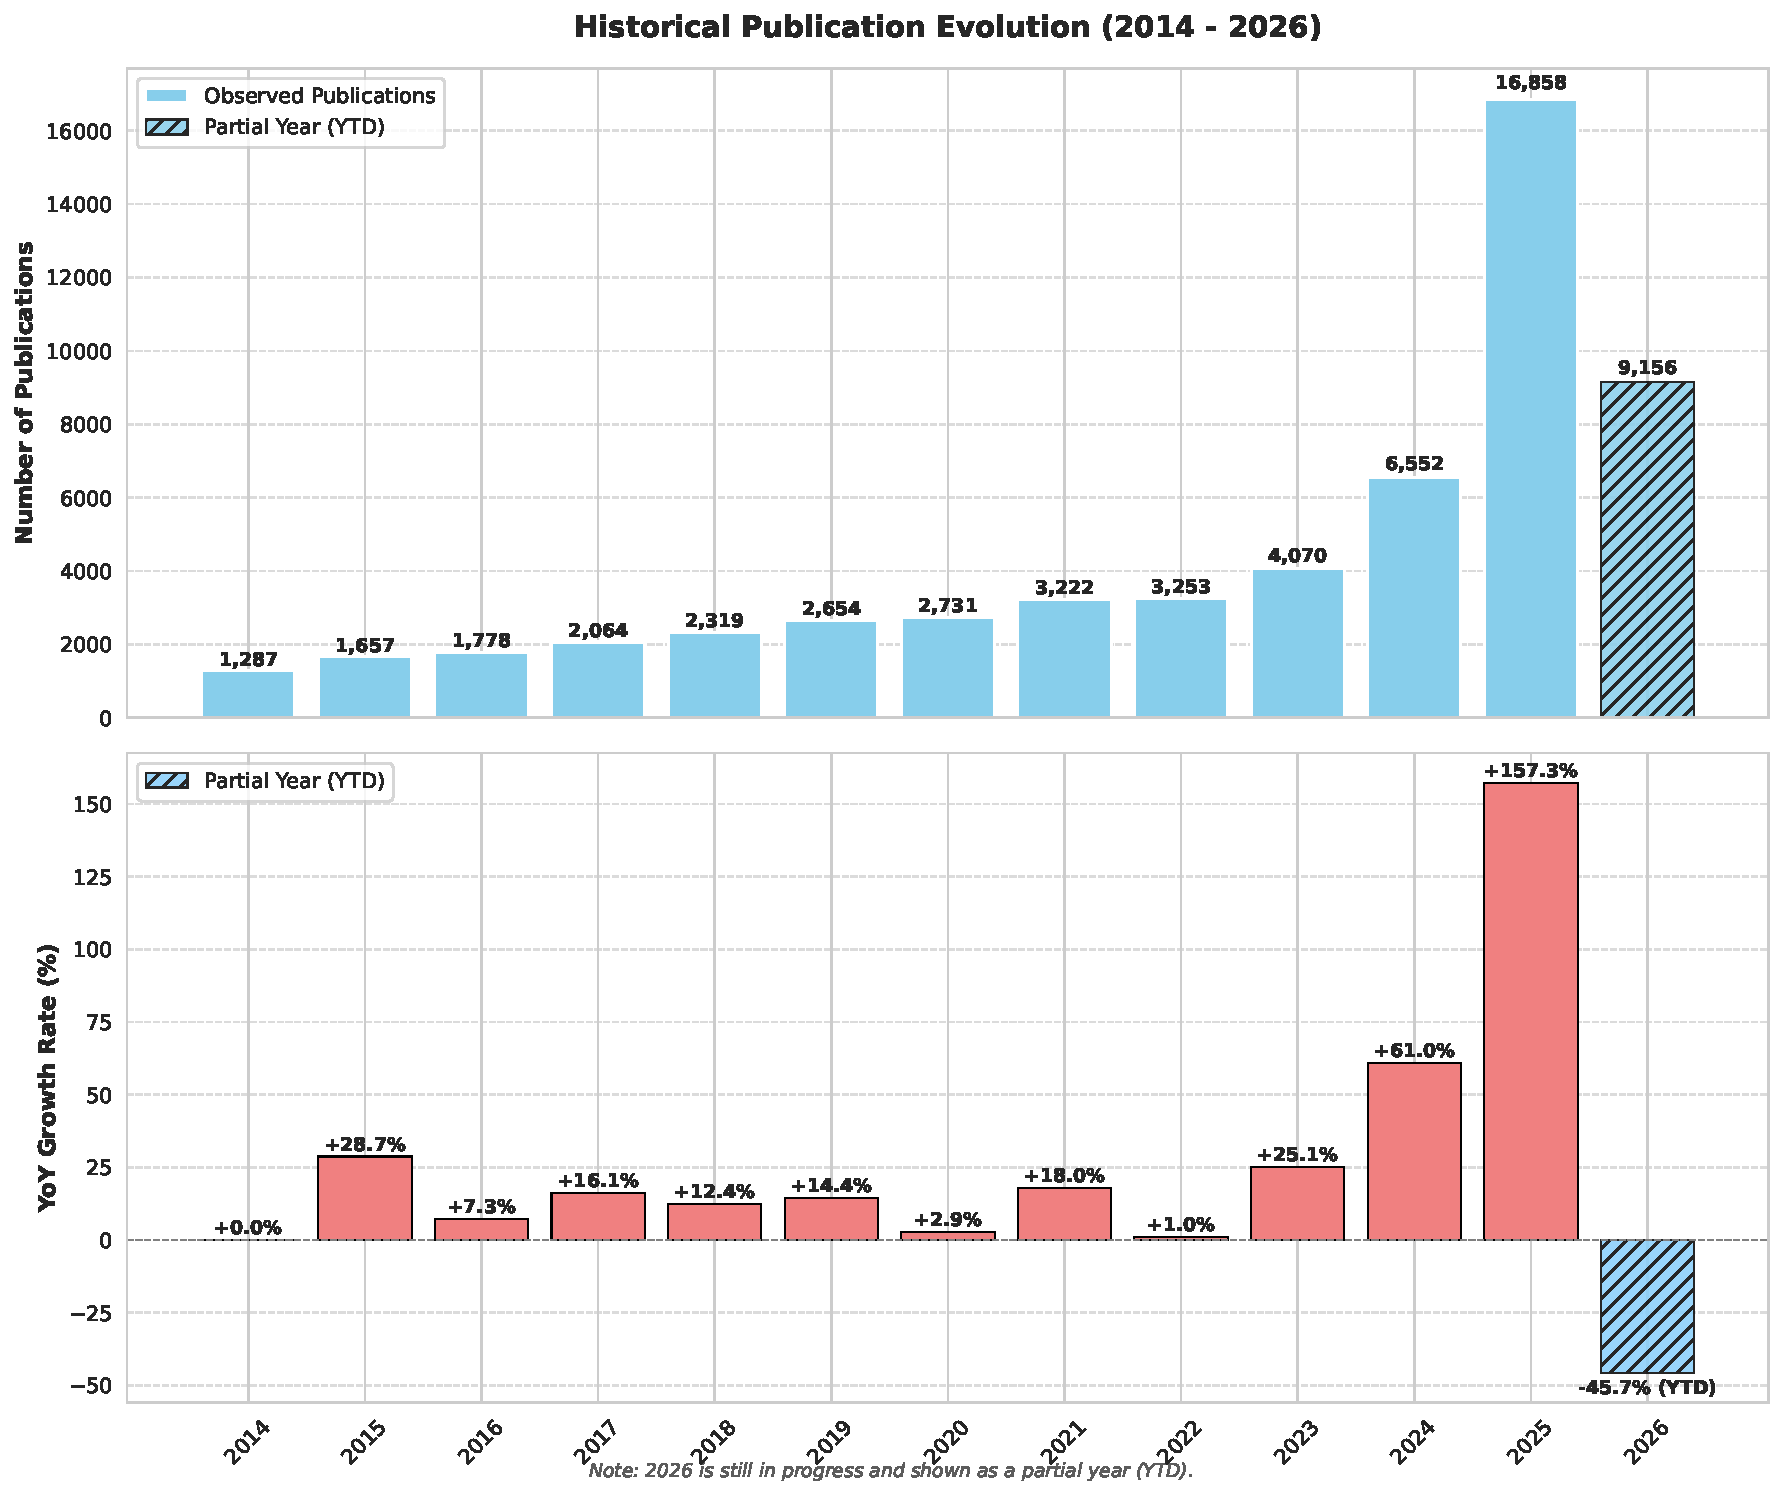
\includegraphics[width=0.72\linewidth]{Figure_1.pdf}}{}
    \caption{Publication Count and Annual Growth}
    \label{fig:pubCountGrowth}
    \vspace{1em}
    \IfFileExists{figures/annual_technique_trajectories.pdf}{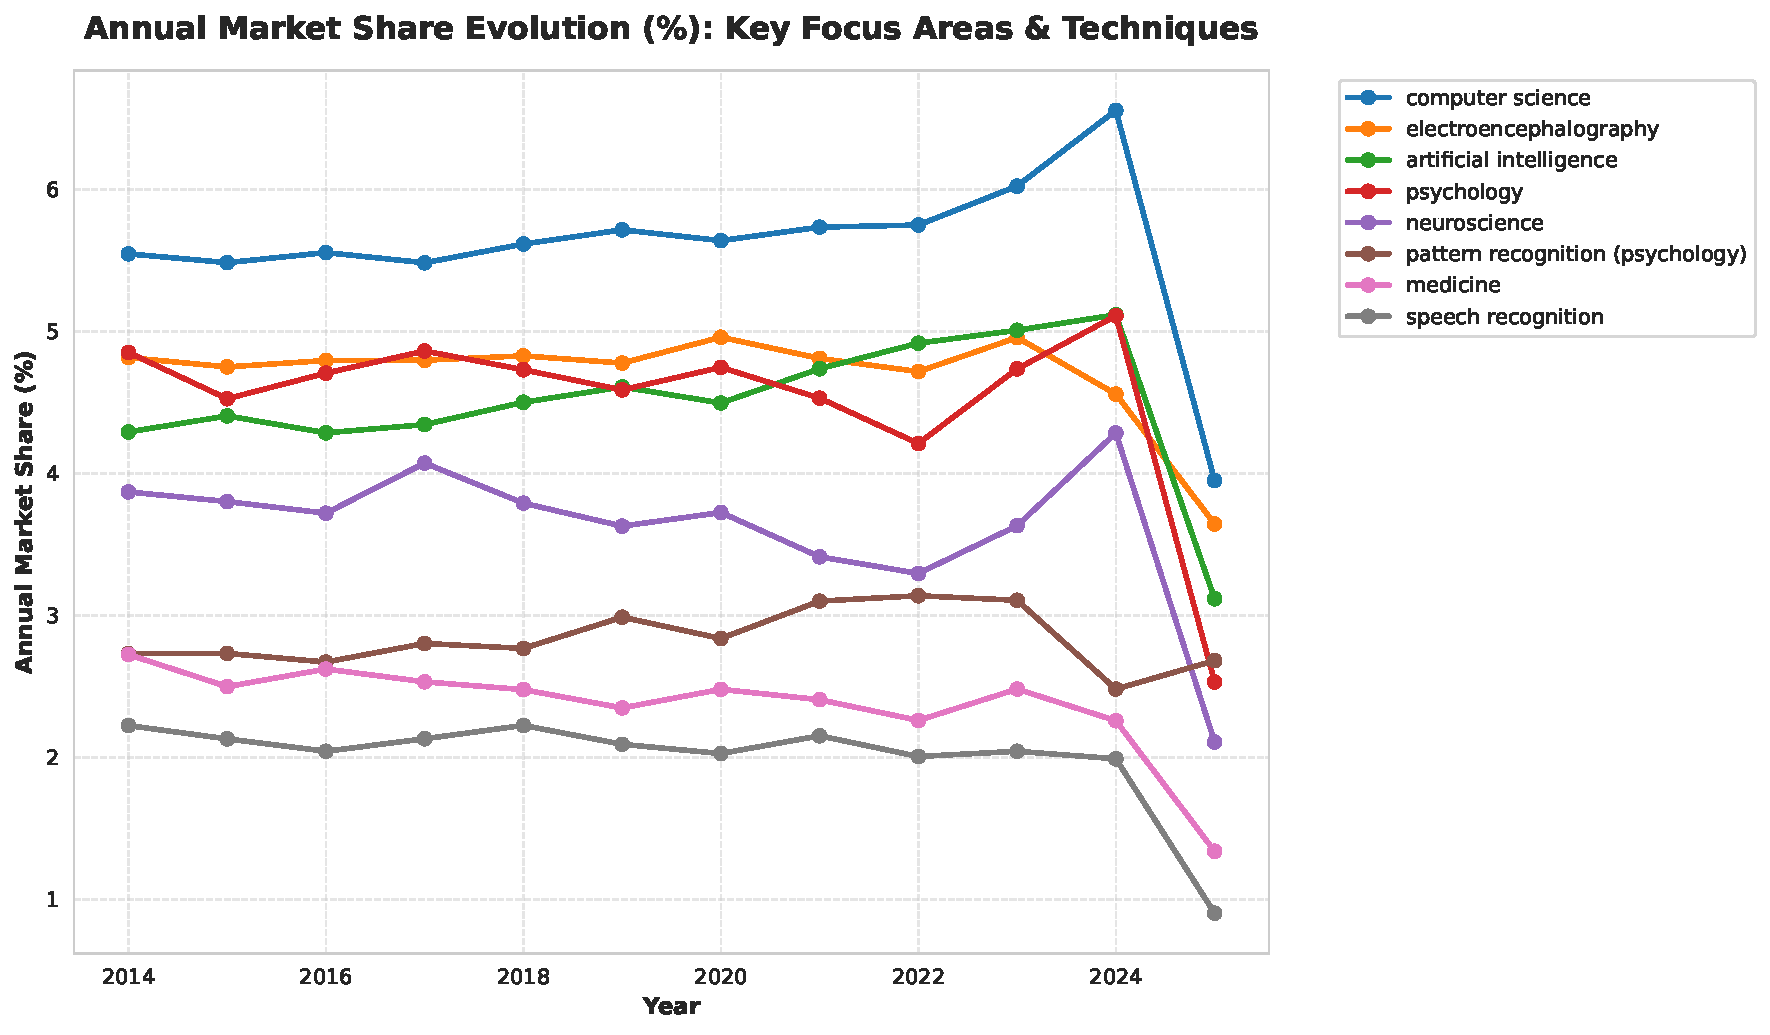
\includegraphics[width=0.72\linewidth]{annual_technique_trajectories.pdf}}{}
    \caption{Annual Market Share Evolution of Key Focus Areas and Techniques}
    \label{fig:technique_trajectories}
\end{figure}

Figure~\ref{fig:technique_trajectories} decomposes the same growth into disciplinary focus areas, documenting the migration of EEG-noise research across computer science, neuroscience, psychology, and clinical medicine over the monitoring window.

Automated rule-based taxonomy categorization of the 57,601 publications reveals that explicit Artifact Filtering \& Removal continues to represent the dominant operational paradigm (95.5\% of the corpus).
\IfFileExists{tables/annex_llm_screening.tex}{\subsection{Deterministic Taxonomy Screening \& Noise Paradigms}
\begin{table}[htbp]
\caption{Keyword-Rule Noise Treatment Paradigm Categorization (clean corpus, $n=57{,}601$)}
\label{tab:llm_screening}
\small
\begin{tabular}{p{0.45\linewidth} r r}
\toprule
\textbf{Noise Treatment Paradigm} & \textbf{Papers} & \textbf{Share (\%)} \\
\midrule
Artifact Filtering \& Removal & 55,011 & 95.5\% \\
General BCI Analysis & 1,341 & 2.3\% \\
Robust Latent Decoding & 731 & 1.3\% \\
Noise-as-Information & 518 & 0.9\% \\
\bottomrule
\end{tabular}
\end{table}}{}

Deterministic classification of the full clean corpus (Table~\ref{tab:llm_screening}) confirms the imbalance: 95.5\% artifact filtering and removal, 2.3\% general analysis, 1.3\% robust latent decoding, and 0.9\% noise-as-information.

\subsection{AI Content Analysis, BERTopic \& Rule-Based Noise Treatment Paradigms}
Figure~\ref{fig:bertopic_clusters} highlights the dominant thematic clusters extracted via BERTopic, revealing application-led pillars in emotion recognition ($T_0$, 1,103 papers), seizure detection ($T_1$, 820 papers), and motor-imagery spatial filtering ($T_2$, 642 papers).

Table~\ref{tab:bertopic_clusters} presents the quantitative decomposition across two distinct analytical tiers: foundational high-volume macro-themes (Panel~A) and specialized frontier micro-clusters (Panel~B). The density-based clustering partitioned 61.1\% ($n=35{,}173$) of the corpus into 553 cohesive, high-confidence thematic micro-clusters. The unclustered background rate of 38.9\% ($n=22{,}428$ in Topic~$-1$) safely isolates boundary documents, highly heterogeneous multi-system medical studies, and broad reviews, ensuring that identified themes represent true semantic density peaks rather than forced partitions. 

Expanding the clean corpus to 57,601 records thickened semantic coordinates across specialized subfields, allowing fine-grained technical frontiers to cross HDBSCAN's density threshold ($\text{min\_cluster\_size}=10$) without inflating macro-cluster noise. As highlighted in Panel~B, these newly resolved frontiers capture critical hardware and algorithmic specializations, including analog front-end (AFE) impedance dynamics ($T_{23}$, $n=236$), neonatal ICU amplitude-integrated EEG ($T_{24}$, $n=235$), invasive stereoelectroencephalography ($T_{36}$, $n=207$), state-space Kalman filtering ($T_{42}$, $n=182$), TMS artifact suppression ($T_{43}$, $n=181$), generative artifact reconstruction via GANs ($T_{91}$, $n=97$), in-ear wearables ($T_{212}$, $n=42$), deep graph convolutional transformers ($T_{432}$, $n=16$), generative diffusion denoising ($T_{523}$, $n=11$), and aperiodic $1/f$ neural timescale dynamics ($T_{532}$, $n=11$).

\begin{figure}[htbp]
    \centering
    \IfFileExists{figures/Figure_20.pdf}{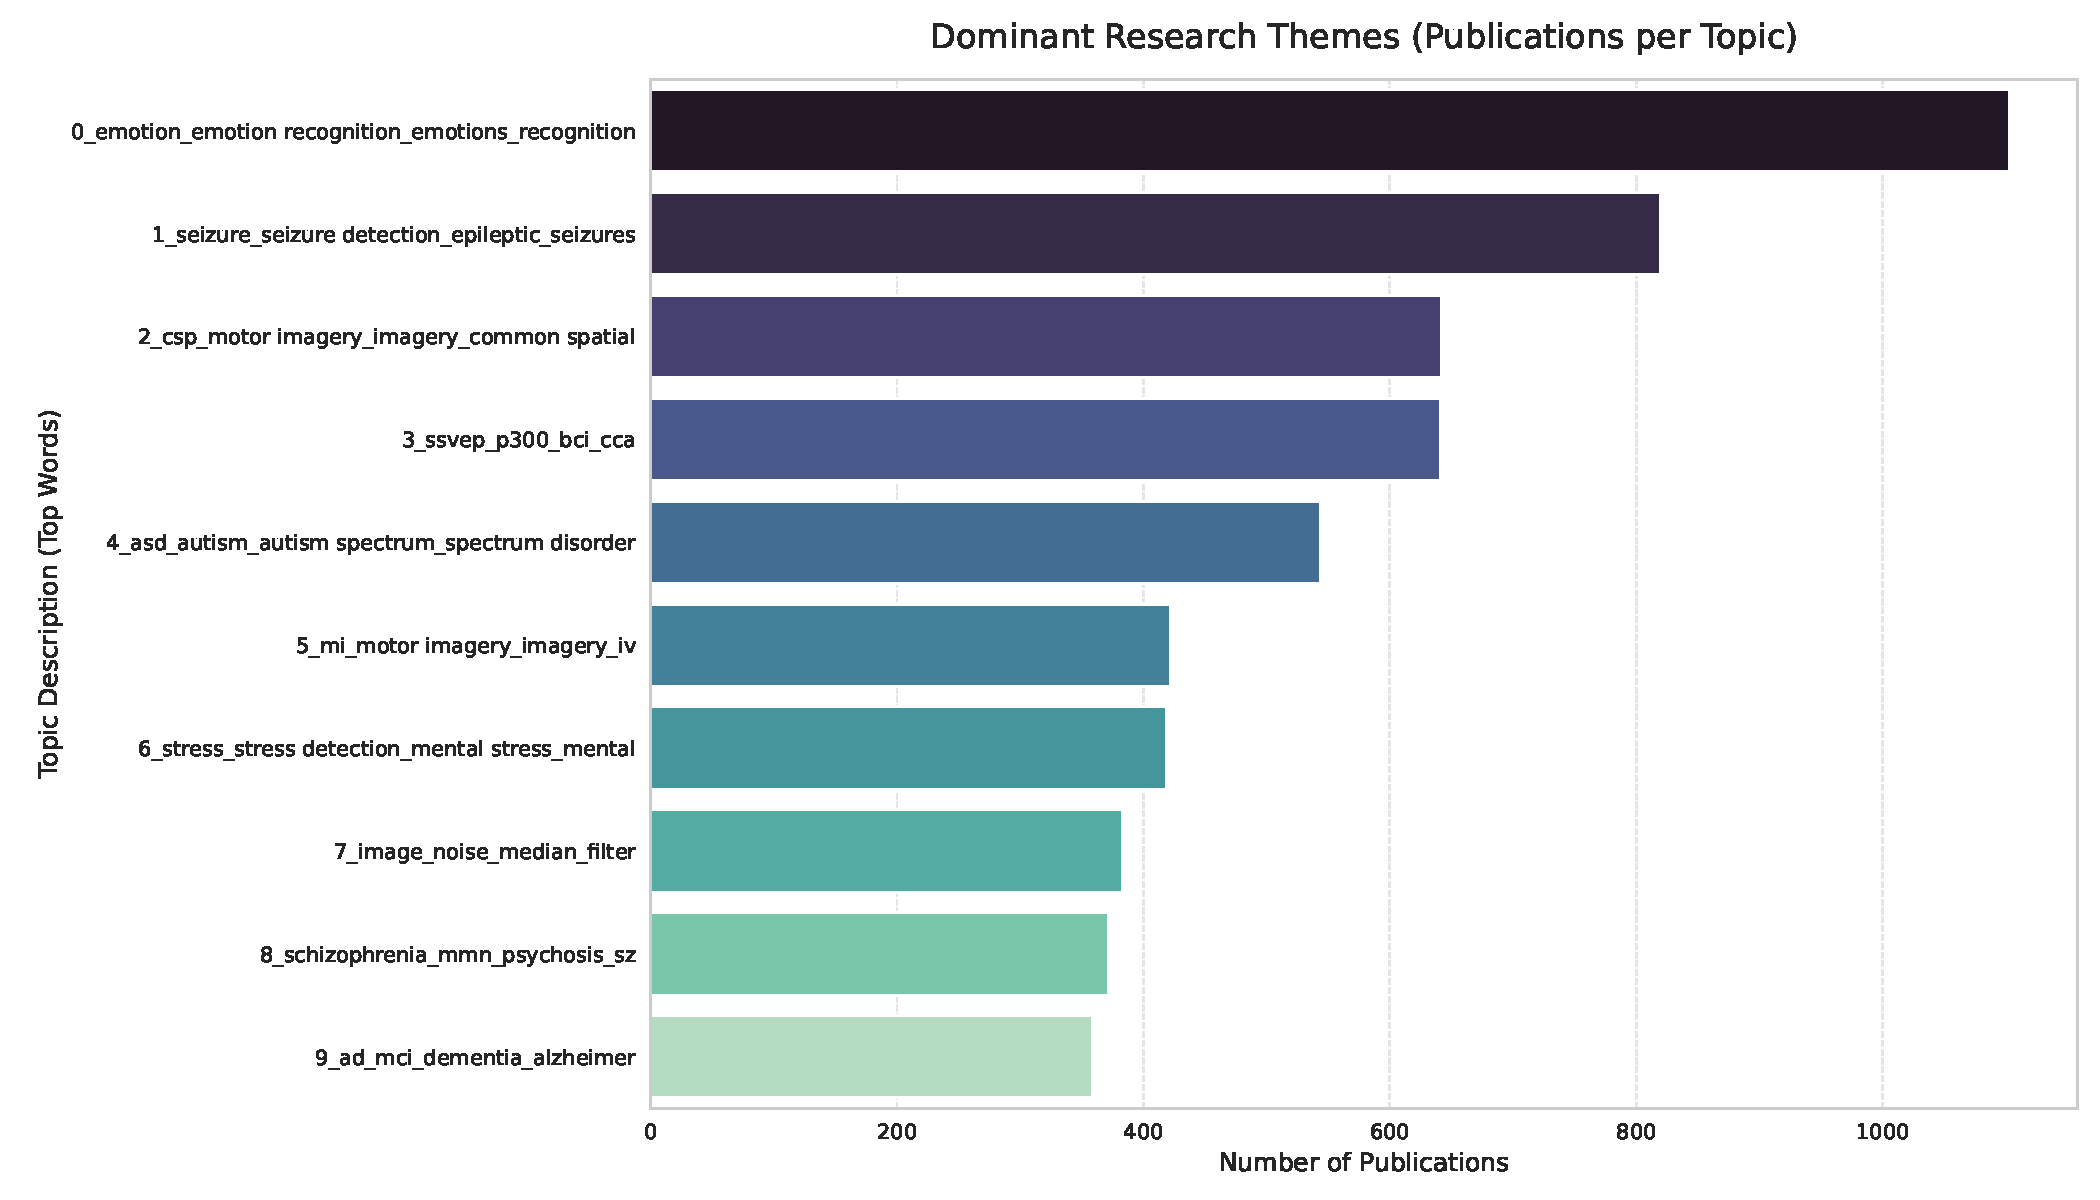
\includegraphics[width=0.72\linewidth]{Figure_20.pdf}}{}
    \caption{Discovered BERTopic Thematic Clusters and Keyword Scores}
    \label{fig:bertopic_clusters}
    \vspace{1em}
    \IfFileExists{figures/Figure_25.pdf}{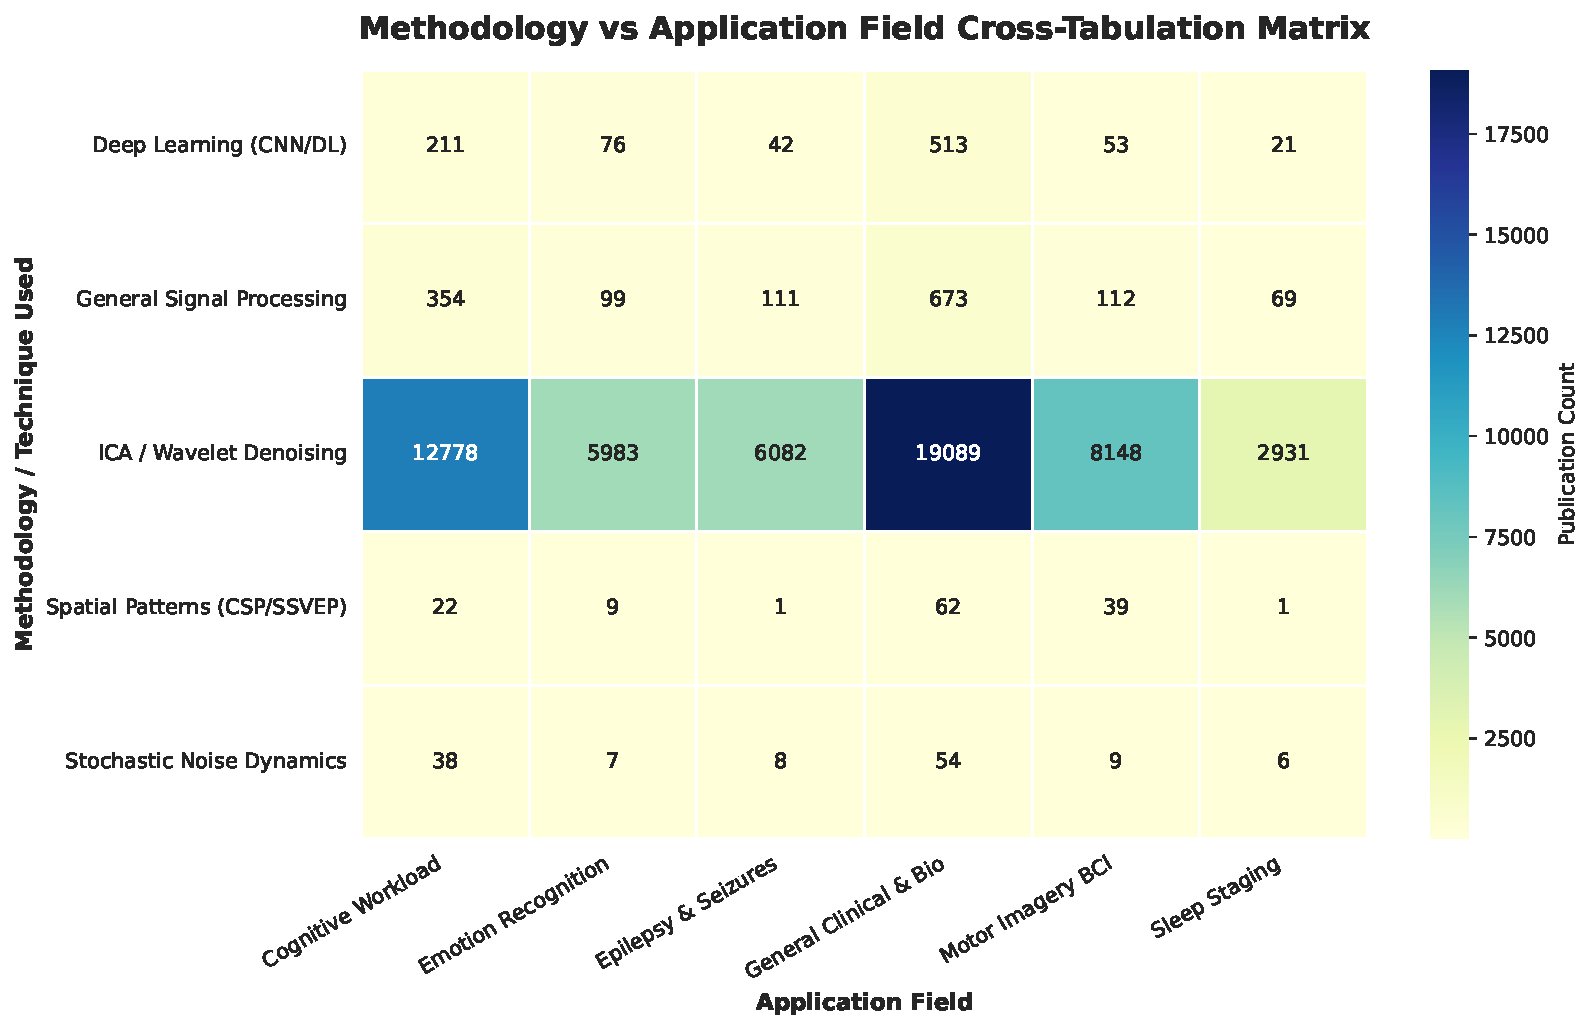
\includegraphics[width=0.72\linewidth]{Figure_25.pdf}}{}
    \caption{Methodology vs Application Field Cross-Tabulation Bipartite Matrix}
    \label{fig:method_application_matrix}
\end{figure}

Figure~\ref{fig:method_application_matrix} cross-tabulates these methodologies against application domains. Classical ICA and Wavelet denoising are overwhelmingly applied in General Clinical contexts (29,375 papers) to maintain interpretability. Deep-learning (CNN/DL) methods remain a small minority overall (786 papers, 1.6\%), concentrating in general-clinical (624 papers) and emotion-recognition (65 papers) applications, bypassing manual component pruning entirely (paired with the BERTopic overview in Figure~\ref{fig:bertopic_clusters}).
Decomposing the same cross-tabulation into three complete-year epochs (Figure~\ref{fig:method_application_epochs}) shows the application rows diverging over time, most visibly in the motor-imagery row, where spatial-pattern shares fall from 29.3\% (2014--2017) to 6.8\% (2022--2025).

\begin{figure}[htbp]
    \centering
    \IfFileExists{figures/method_application_multi_epoch.pdf}{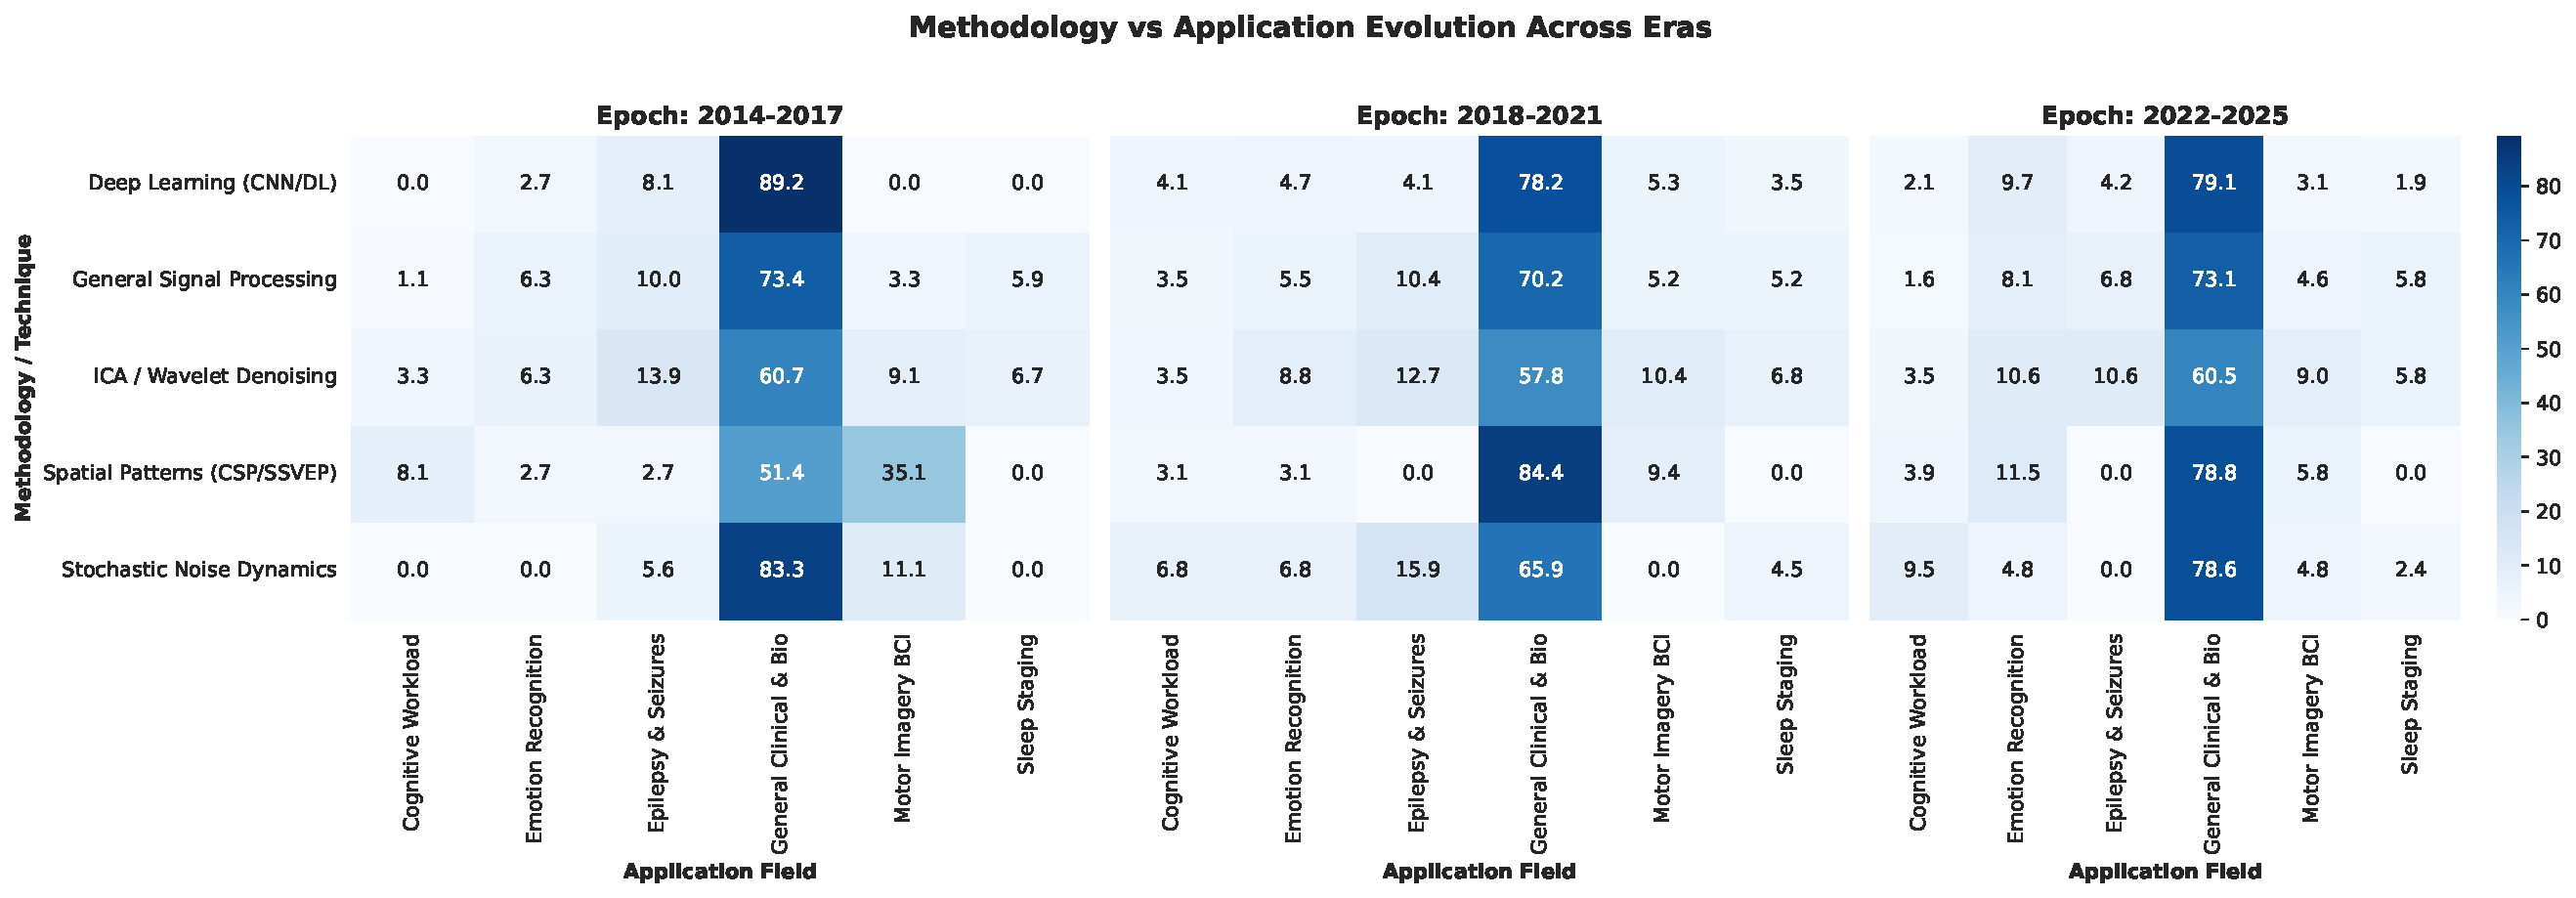
\includegraphics[width=0.72\linewidth]{method_application_multi_epoch.pdf}}{}
    \caption{Methodology vs Application Evolution Across Epochs (2014--2017, 2018--2021, 2022--2025)}
    \label{fig:method_application_epochs}
\end{figure}

\subsection{Scientific Temporal Dynamics \& Paradigm Shifts (\texorpdfstring{$\Delta$}{Delta} Analysis)}
The market share deltas shown in Figure~\ref{fig:temporal_delta_shifts} quantify the temporal paradigm shift between the baseline (2014--2019) and modern (2020--2025) epochs. Deep learning ($\Delta = +1.30\%$), convolutional neural network ($\Delta = +0.69\%$), and artificial neural network ($\Delta = +0.62\%$) exhibit the largest positive momentum, displacing broad disciplinary terms like psychology ($\Delta = -0.81\%$) and neuroscience ($\Delta = -0.71\%$).

\begin{figure}[htbp]
    \centering
    \IfFileExists{figures/Figure_15.pdf}{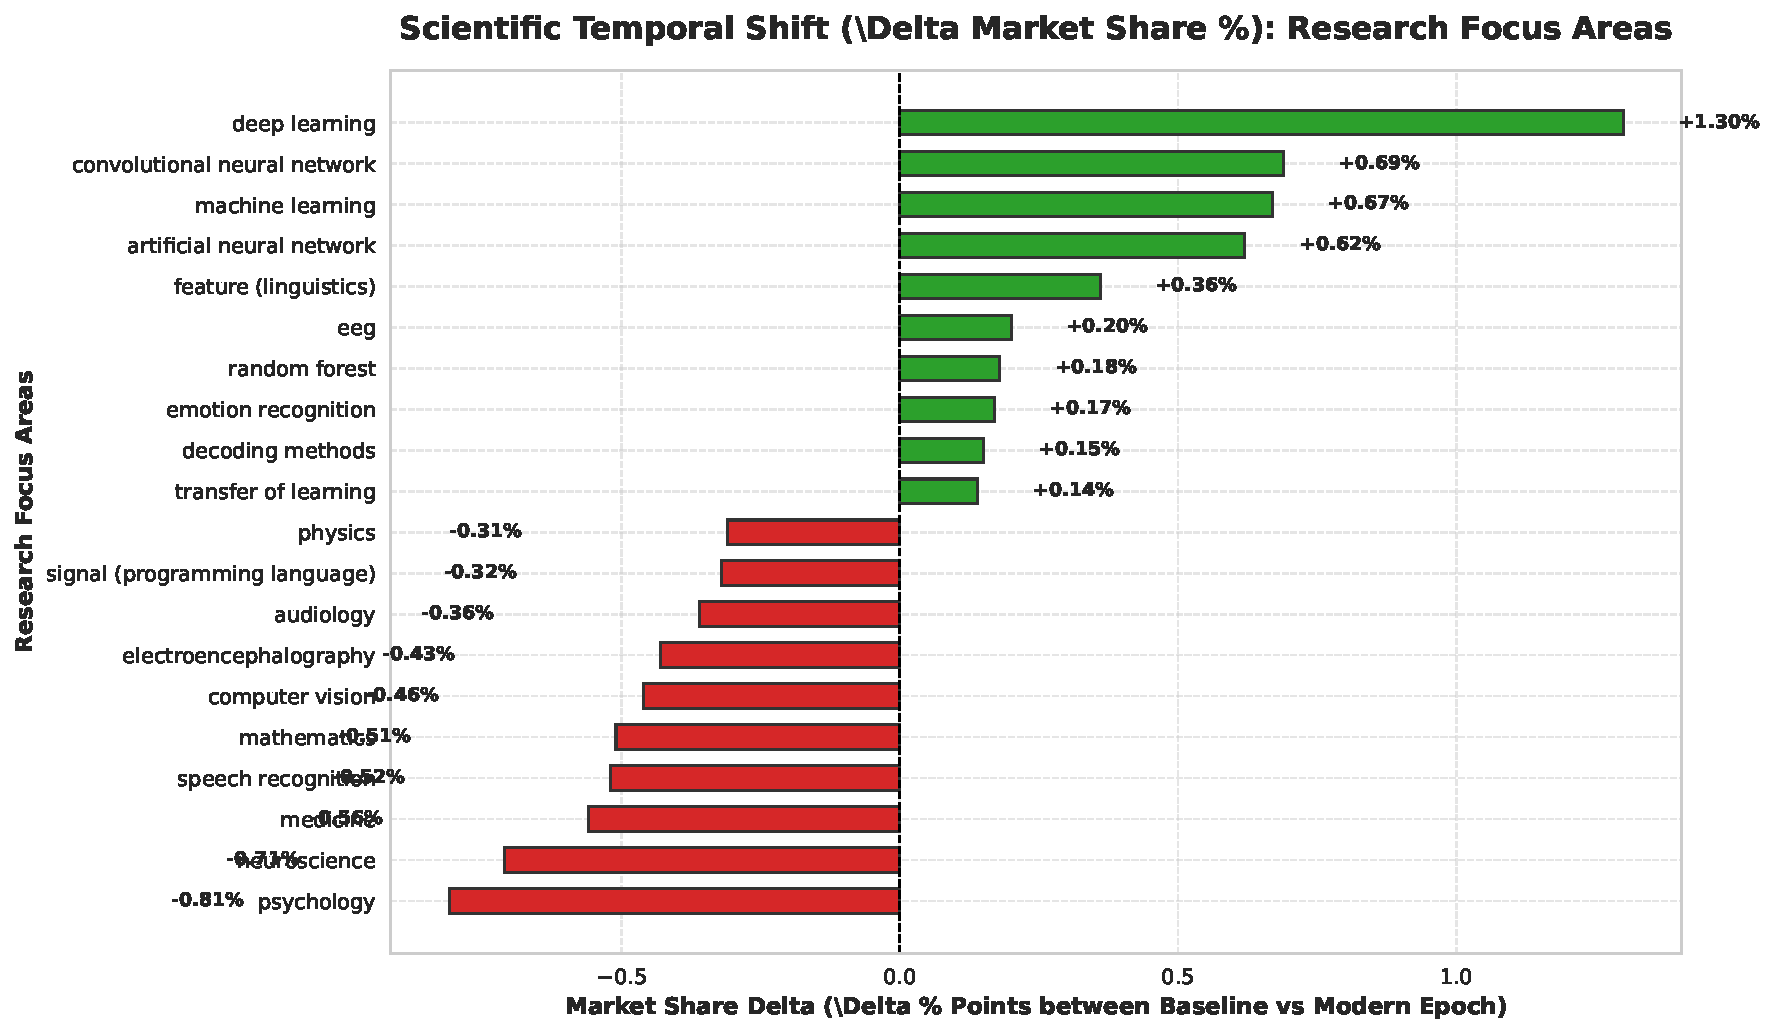
\includegraphics[width=0.72\linewidth]{Figure_15.pdf}}{}
    \caption{Scientific Market Share Deltas ($\Delta$ \%) Between Baseline vs Modern Epochs}
    \label{fig:temporal_delta_shifts}
\end{figure}

\subsection{Authorship and Community Analysis}
Figure~\ref{fig:network_graph} maps the Louvain co-authorship communities, identifying dense collaborative clusters structured around leading neuroengineering hubs working on signal processing.

\begin{figure}[htbp]
    \centering
    \IfFileExists{figures/Figure_8.pdf}{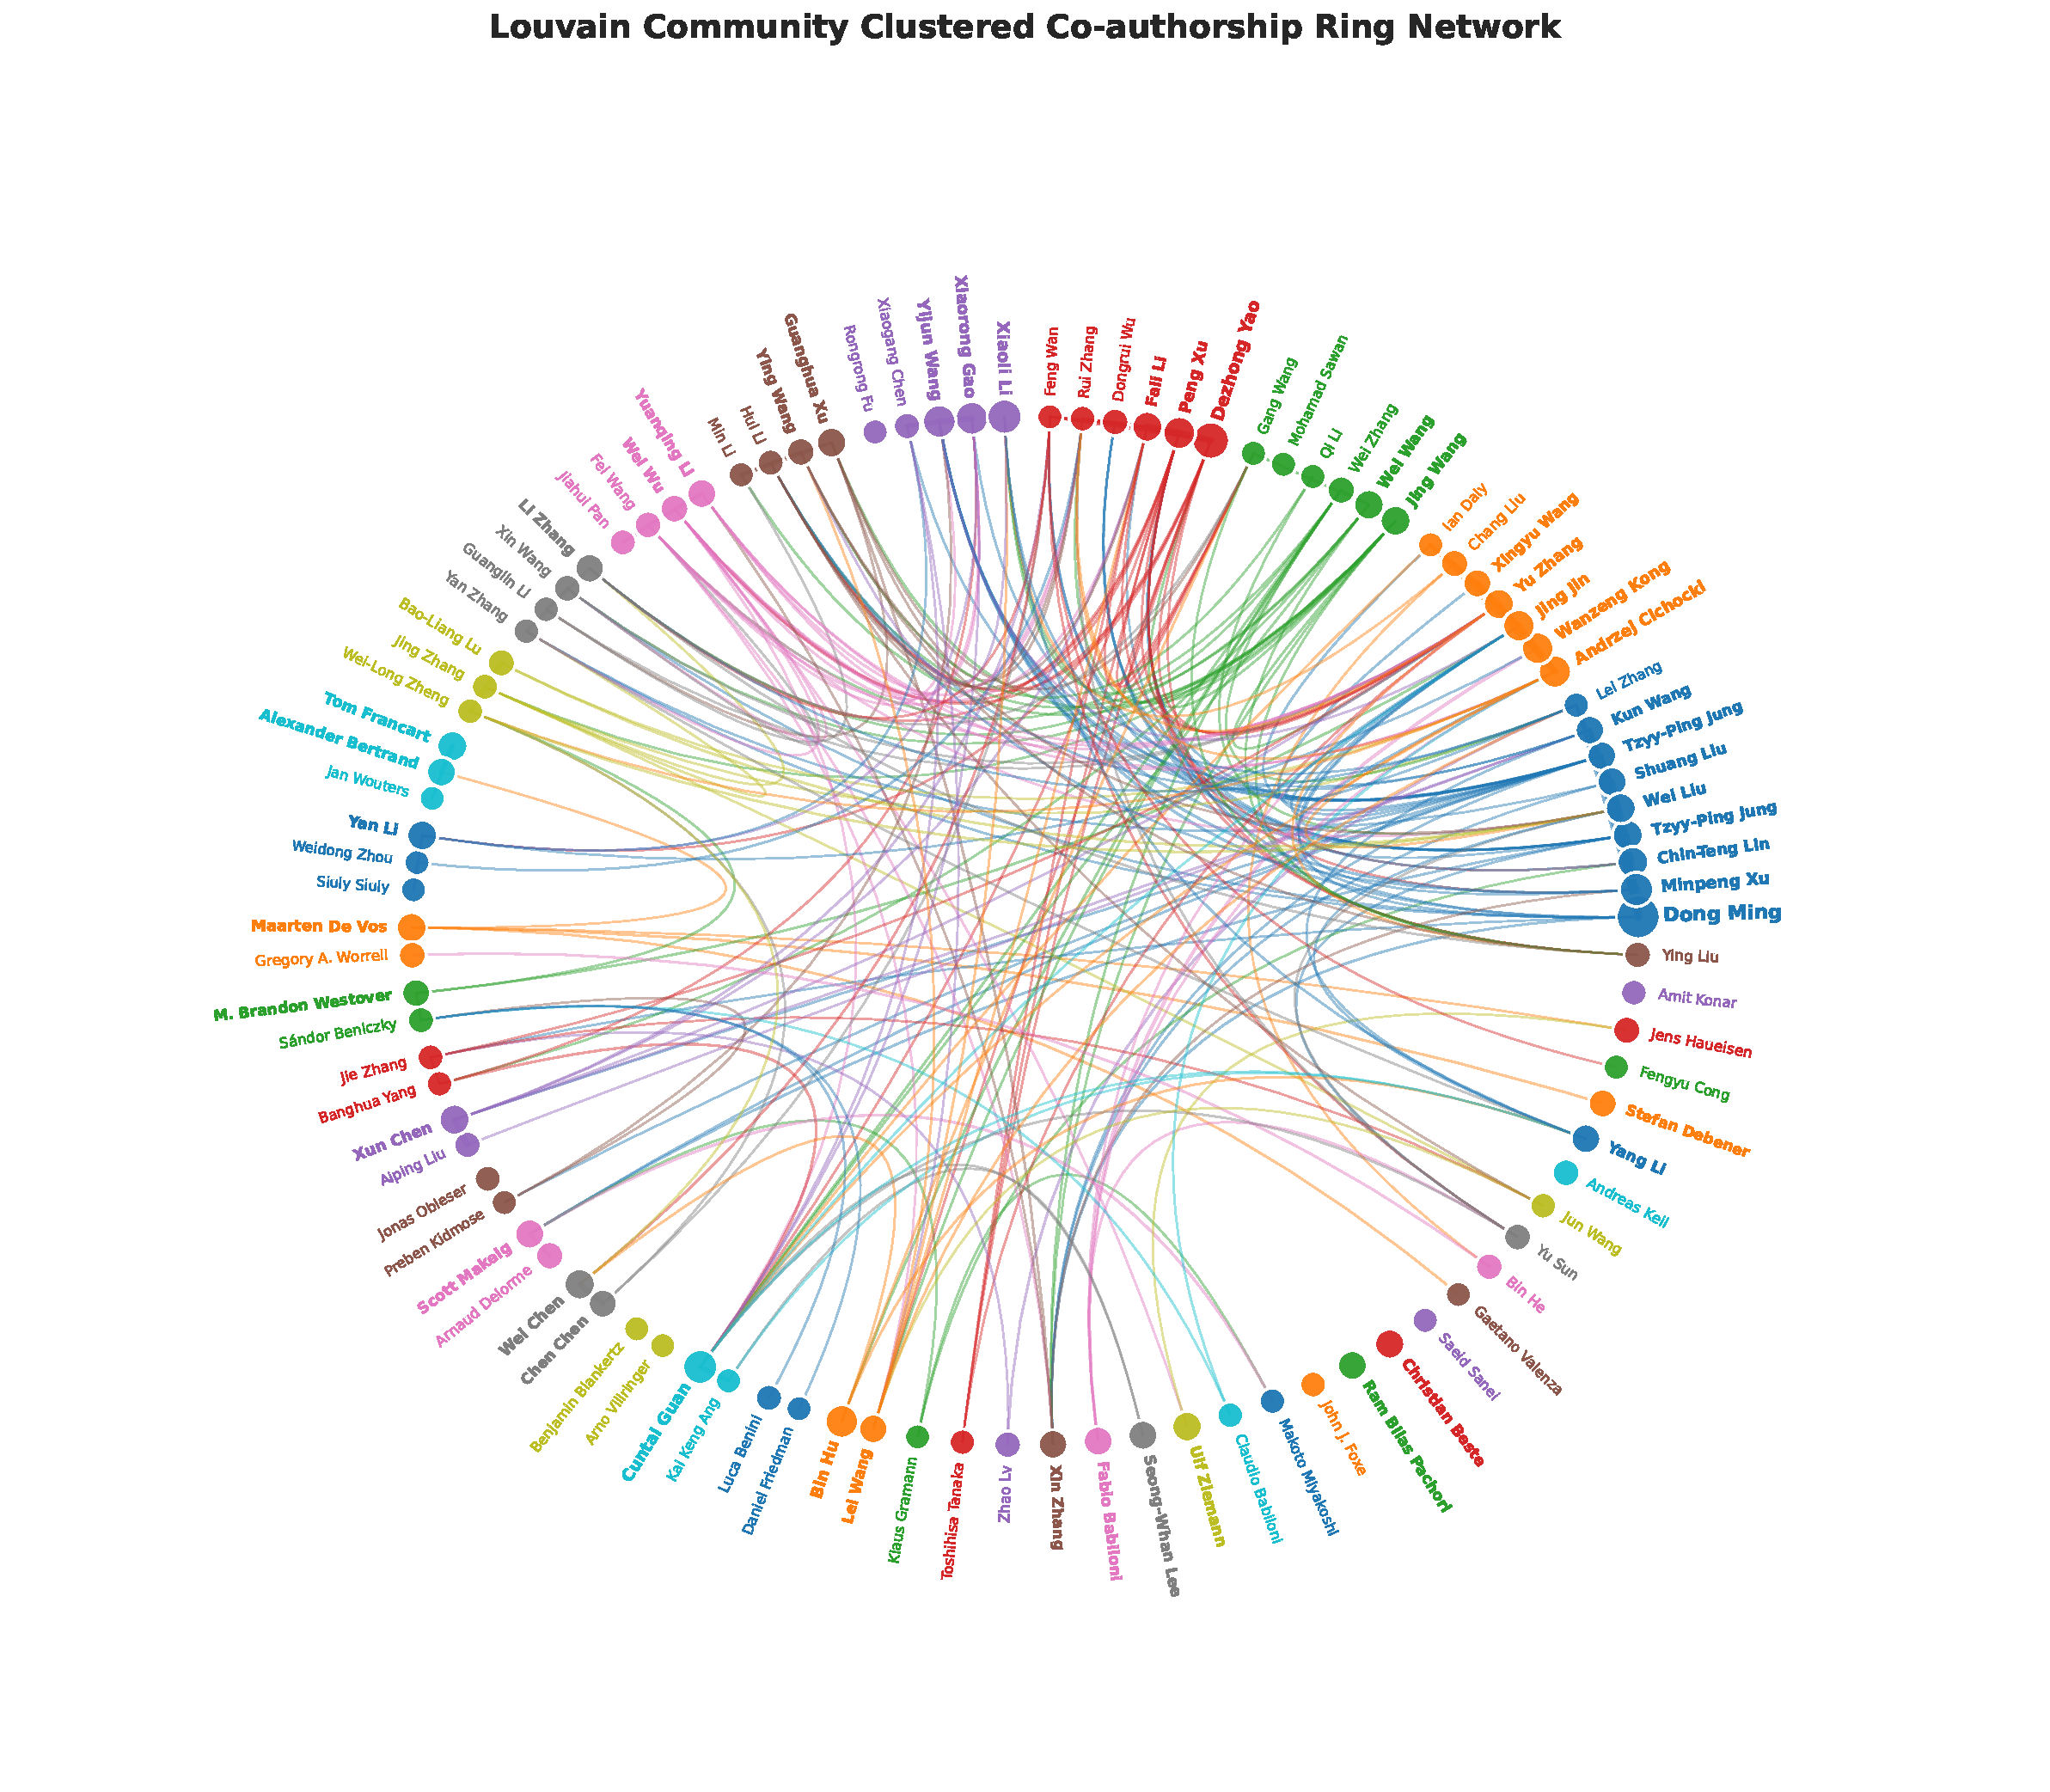
\includegraphics[width=0.72\linewidth]{Figure_8.pdf}}{}
    \caption{Louvain Community Clustered Co-Authorship Ring Network}
    \label{fig:network_graph}
    \vspace{1em}
    \IfFileExists{figures/Figure_10.pdf}{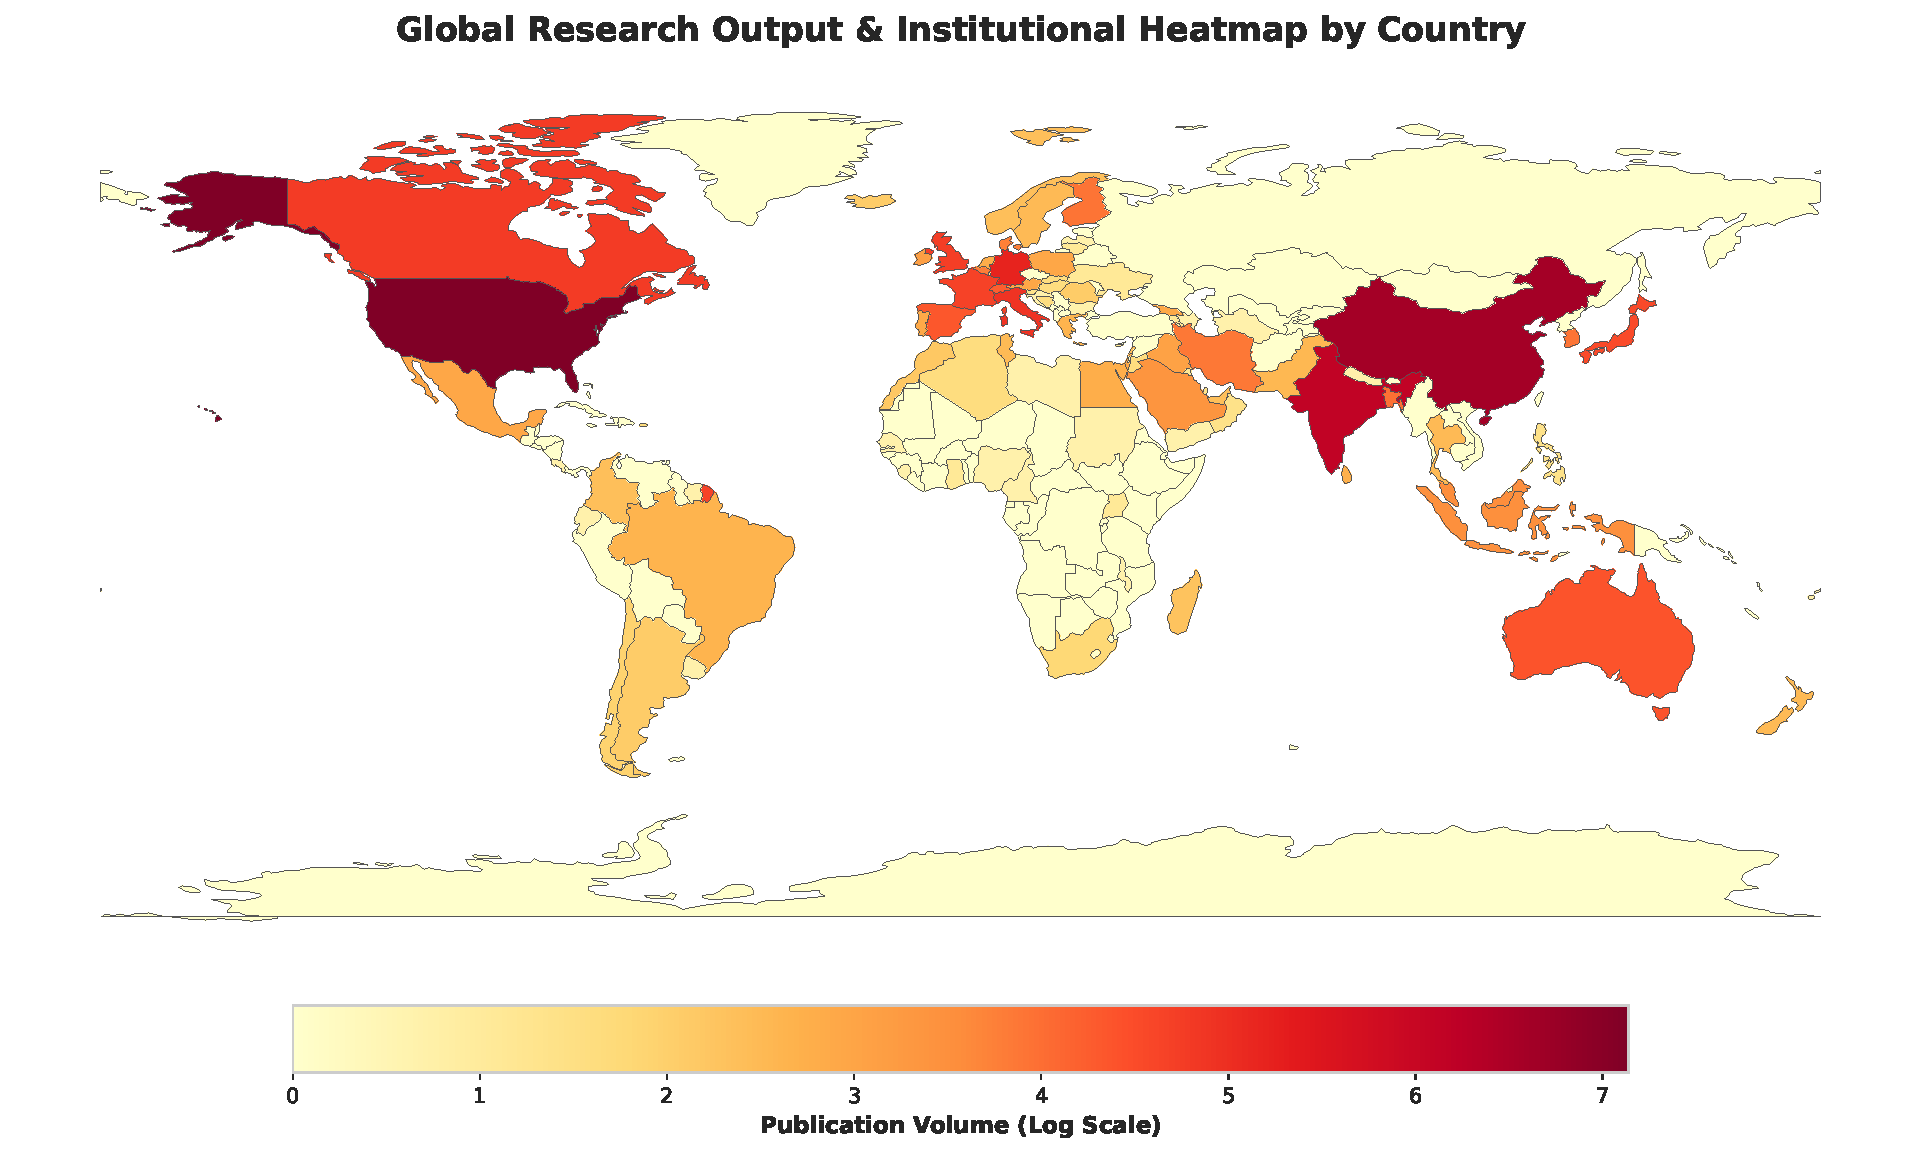
\includegraphics[width=0.72\linewidth]{Figure_10.pdf}}{}
    \caption{Global Institutional Research Heatmap by Country}
    \label{fig:country_world_map}
\end{figure}

The geographic distribution in Figure~\ref{fig:country_world_map} (paired with the collaboration network above) demonstrates an ongoing global redistribution of research output. While the United States maintains the highest cumulative volume, surging publication growth rates in China and India reflect expanding research capacity and heightened activity in deep learning pipelines and mobile EEG hardware.

\subsection{Reference-Based Analysis}
\subsubsection{Co-Citation Network}
Figure~\ref{fig:cocitation_graph} illustrates the reference co-citation network, ranked by co-citation count to highlight the foundational backbone of the domain. The graph exposes a dual-hub structure, with a BSS cluster led by EEGLAB \cite{delorme2004eeglab} and FieldTrip \cite{oostenveld2011fieldtrip}, and an end-to-end convolutional cluster led by EEGNet \cite{lawhern2018eegnet} and DeepConvNet \cite{schirrmeister2017deep}.

\begin{figure}[htbp]
    \centering
    \IfFileExists{figures/Figure_5.pdf}{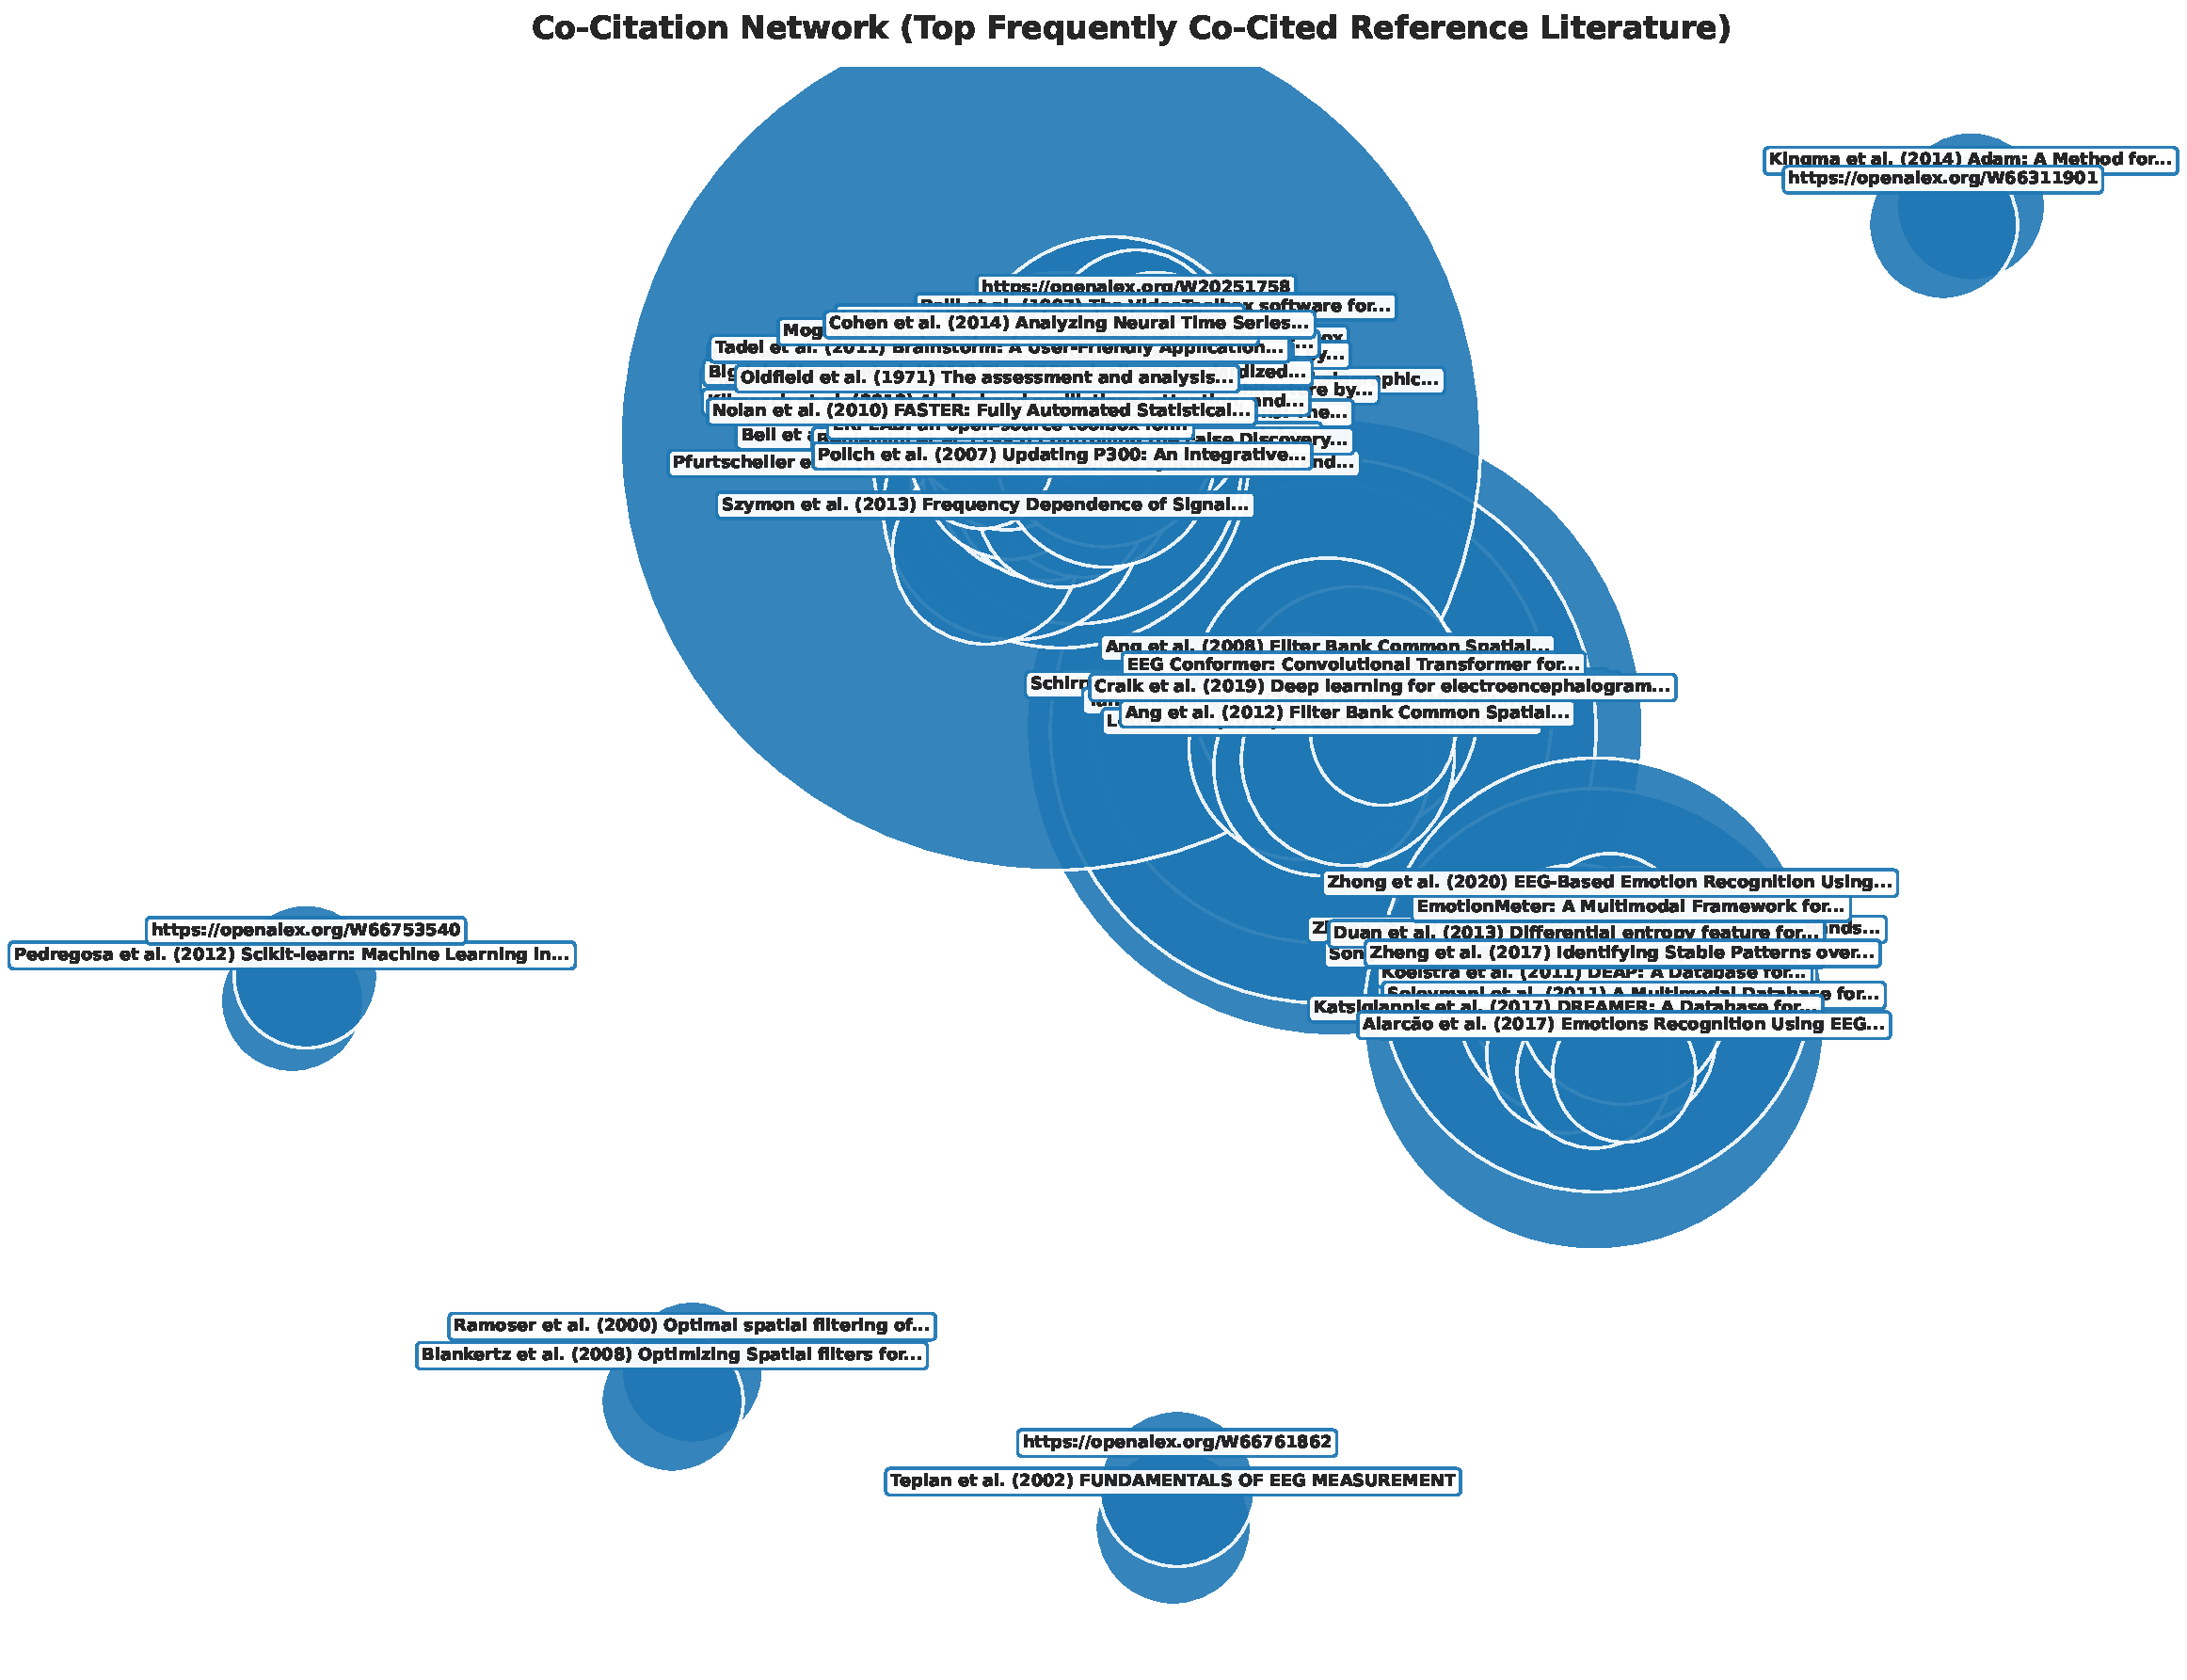
\includegraphics[width=0.72\linewidth]{Figure_5.pdf}}{}
    \caption{Reference Co-Citation Network Graph}
    \label{fig:cocitation_graph}
\end{figure}
\IfFileExists{tables/tab_top_references_pagerank.tex}{\begin{table}[htbp]
\caption{Top 20 Most Referenced Landmark Publications}
\label{tab:top_references_pagerank}
\footnotesize
\begin{tabular}{p{0.75\linewidth} r}
\toprule
\textbf{Landmark Reference Publication} & \textbf{Citations} \\
\midrule
\href{https://doi.org/10.1016/j.jneumeth.2003.10.009}{Delorme et al. (2004) EEGLAB: an open source...} & 239,390 \\
\href{https://doi.org/10.1155/2011/156869}{Oostenveld et al. (2010) FieldTrip: Open Source Software...} & 99,762 \\
\href{https://doi.org/10.1016/j.jneumeth.2007.03.024}{Maris et al. (2007) Nonparametric statistical testing of...} & 68,875 \\
\href{https://doi.org/10.1088/1741-2552/aace8c}{Lawhern et al. (2018) EEGNet: a compact convolutional...} & 67,032 \\
\href{https://doi.org/10.1016/s1388-2457(99)00141-8}{Pfurtscheller et al. (1999) Event-related EEG/MEG synchronization and...} & 60,044 \\
\href{https://doi.org/10.1002/hbm.23730}{Schirrmeister et al. (2017) Deep learning with convolutional...} & 55,031 \\
\href{https://doi.org/10.1016/s0165-0173(98)00056-3}{Klimesch et al. (1999) EEG alpha and theta...} & 54,526 \\
\href{https://doi.org/10.1109/t-affc.2011.15}{Koelstra et al. (2011) DEAP: A Database for...} & 46,822 \\
\href{https://doi.org/10.1016/j.clinph.2007.04.019}{Polich et al. (2007) Updating P300: An integrative...} & 43,527 \\
\href{https://doi.org/10.3389/fnins.2013.00267}{Gramfort et al. (2013) MEG and EEG data...} & 42,593 \\
\href{https://doi.org/10.1016/j.neuroimage.2019.05.026}{Pion-Tonachini et al. (2019) ICLabel: An automated electroencephalographic...} & 41,164 \\
\href{https://doi.org/10.1111/j.2517-6161.1995.tb02031.x}{Benjamini et al. (1995) Controlling the False Discovery...} & 40,283 \\
\href{https://doi.org/10.1016/s1388-2457(02)00057-3}{Wolpaw et al. (2002) Brain–computer interfaces for communication...} & 39,079 \\
\href{https://doi.org/10.1016/j.tics.2012.10.007}{Klimesch et al. (2012) Alpha-band oscillations, attention, and...} & 37,662 \\
\href{https://doi.org/10.1016/j.brainresrev.2006.06.003}{Klimesch et al. (2006) EEG alpha oscillations: The...} & 37,239 \\
\href{https://doi.org/10.1109/tamd.2015.2431497}{Zheng et al. (2015) Investigating Critical Frequency Bands...} & 35,339 \\
\href{https://doi.org/10.3389/fnhum.2010.00186}{Jensen et al. (2010) Shaping Functional Architecture by...} & 35,261 \\
\href{https://doi.org/10.1163/156856897x00357}{Brainard et al. (1997) The Psychophysics Toolbox} & 33,841 \\
\href{https://doi.org/10.1016/0028-3932(71)90067-4}{Oldfield et al. (1971) The assessment and analysis...} & 33,131 \\
\href{https://doi.org/10.1088/1741-2552/aab2f2}{Lotte et al. (2018) A review of classification...} & 33,119 \\
\bottomrule
\end{tabular}
\end{table}}{}
Complementary bibliographic coupling pairs cluster around the same challenging noise domains, including high-amplitude electromagnetic pulses in TMS-EEG \cite{rogasch2014removing, farzan2016characterizing} and methodological spectral parameterization separating aperiodic $1/f^\beta$ background dynamics from true narrowband oscillatory peaks \cite{gerster2022separating, porcaro2026quantifying}.

\section{Discussion}
The bibliometric data shows that traditional artifact removal remains the standard approach across most of the field, accounting for 95.5\% of all reviewed studies. At the same time, newer approaches, such as deep learning models that learn noise-tolerant representations and methods that analyze aperiodic $1/f^\beta$ background activity, are growing rapidly in specific areas like brain--computer interfaces.

\subsection{Waveform Integrity vs.\ Latent-Space Invariance}
The methodological divergence revealed in the bipartite cross-tabulation (Figure~\ref{fig:method_application_matrix}) is fundamentally dictated by clinical versus engineering constraints. In clinical neurology, representing the dominant application context of 29,375 publications, diagnostic evaluation relies on preserving the raw microvolt morphology and phase alignment of physiological waveforms, such as focal epileptiform spike-and-wave discharges, slow-wave delta slowing, and sleep transients. Clinicians and diagnostic certified algorithms require explicit, linear subspace projection like extended Infomax or fastICA \cite{delorme2004eeglab, jung2000removing} because the unmixing matrix $\mathbf{W} = \mathbf{A}^{-1}$ is invertible and visualizable, allowing neurophysiologists to inspect the topographical scalp projection of isolated ocular or cardiac components before approving rejection.

Conversely, closed-loop brain--computer interfaces and mobile neurotechnologies operate under strict runtime latency budgets of 20--50\,ms and restricted electrode montages of 4 to 8 channels. Under these underdetermined conditions where $N_{\text{channels}} \ll N_{\text{sources}}$, classical BSS algorithms fail due to matrix rank deficiency and numerical instability. The rapid rise of compact spatial-temporal architectures, exemplified by models such as EEGNet \cite{lawhern2018eegnet} and DeepConvNet \cite{schirrmeister2017deep}, circumvents explicit unmixing by performing 2D depthwise and separable convolutions directly over raw signals. These architectures treat noise mitigation as an implicit optimization objective, suppressing non-cerebral artifacts that do not co-vary with task labels within latent representations, without requiring separate decomposition steps.

\subsection{Aperiodic Dynamics and Redefining Biological ``Noise''}
A notable conceptual shift within the literature is the emergence of the noise-as-information framework in Paradigm~3. Electrophysiological studies have traditionally focused on narrowband oscillatory rhythms ($\theta, \alpha, \beta, \gamma$), largely treating the underlying broadband decay of the power spectrum as uninformative background noise. However, recent studies identified within the spectral parameterization coupling cluster \cite{gerster2022separating, porcaro2026quantifying} demonstrate the value of explicitly decomposing the power spectrum into an aperiodic background and periodic oscillatory peaks:
\begin{equation}
\text{PSD}(f) = L(f) + \sum_{i} G_i(f)
\end{equation}
where $L(f)$ captures the continuous aperiodic component and $G_i(f)$ denotes Gaussian oscillatory peaks. In this framework, the aperiodic slope $\beta$ reflects collective, scale-free neural activity that correlates with the balance between cortical synaptic excitation and inhibition. 

This decomposition introduces practical implications for signal processing. Standard aggressive preprocessing, such as high-pass filtering above 1\,Hz or wide notch filtering, risks distorting low-frequency phase relationships and altering the aperiodic slope. Recognizing the aperiodic background as a physiological feature rather than pure noise highlights the need for parameterization tools that decouple actual artifactual interference from informative background dynamics.

\subsection{The Latent Shortcut Dilemma}
While end-to-end deep learning pipelines in Paradigm~2 achieve high empirical decoding accuracy on static benchmark datasets, they introduce a substantial risk of shortcut learning. Because deep networks optimize primarily for task classification loss, latent encoders can learn to exploit high-amplitude physiological artifacts, such as micro-saccades or subtle muscle clenching during cognitive effort, as predictive features rather than suppressing them. 

This creates a critical performance gap between offline evaluations and live, closed-loop execution. In real-time deployments, spontaneous movements, postural changes, and electrode impedance drift disrupt the accidental correlations learned during offline training, frequently causing decoders to fail when evaluated online. In clinical monitoring and real-time interfaces, models that appear robust offline can deteriorate across sessions or hardware montages where artifact distributions decouple from genuine neural activity. Hybrid pipelines combining automated, verifiable artifact attenuation like ICLabel \cite{pion2019iclabel} with compact deep spatial decoders provide a much more dependable strategy for practical, live systems.

\subsection{Limitations \& Threats to Validity}
Several bibliometric limitations should be noted. First, although the automated multi-source ingestion protocol across OpenAlex, Semantic Scholar, and Crossref minimized disciplinary bias between medical and engineering venues, unindexed technical reports were excluded; no explicit language filter was applied, but audit sampling shows 99.8\% of abstracts are English. Second, while deterministic rule-based screening achieved complete taxonomic categorization, edge-case papers spanning multiple paradigms were categorized by primary thematic contribution. Finally, the density-based HDBSCAN topic model deliberately preserved a 38.9\% unclustered residual (Topic $-1$), reflecting highly heterogeneous clinical case studies rather than forced thematic clustering.

\section{Conclusion}
Over the 2014--2026 monitoring period, EEG noise treatment has expanded beyond manual filtering and linear blind source separation into automated, data-driven representation learning. Deep learning models have redefined state-of-the-art decoding by embedding noise invariance directly within spatial-temporal layers. Addressing future deployment demands will require hybrid pipelines that combine automated artifact suppression with interpretable, noise-robust architectures suitable for real-time mobile neurotechnology.

\section*{CRediT Authorship Contribution Statement}
\textbf{João Garcia Farinha:} Conceptualization, Methodology, Software, Data Curation, Formal Analysis, Investigation, Visualization, Writing -- original draft. \textbf{Carlos Duarte:} Conceptualization, Supervision, Writing -- review \& editing.

\section*{Declaration of Competing Interest}
The authors declare that they have no known competing financial interests or personal relationships that could have appeared to influence the work reported in this paper.

\section*{Ethics Statement}
This study is a secondary computational science-mapping and bibliometric analysis of public, open-access bibliographic metadata (OpenAlex, Semantic Scholar, Crossref). No human participants, human data, or animal subjects were involved and no new measurements were performed. Ethical approval and informed consent were therefore not required. SAGER sex and gender reporting guidelines are not applicable as no participant-level data were analyzed.

\section*{Data and Code Availability}
The harmonized 57,601-publication bibliometric corpus, BERTopic neural clustering outputs, country publication trajectories, and science-mapping network data supporting this review are openly available on Zenodo~\cite{zenodo2026eeg}.
% TODO(author): upload v2 of the Zenodo record matching the 57,601 clean corpus before submission.
Computational pipelines and replication scripts are accessible via OpenSciencePipe at \url{https://github.com/JohnGF/OpenSciencePipe}.

\section*{Declaration of generative AI and AI-assisted technologies in the manuscript preparation process}
During the preparation of this work the authors used an AI-assisted coding environment in order to convert the manuscript to the Elsevier LaTeX template, format figures and annex tables from the cleaned corpus, and polish document layout. After using this tool, the authors reviewed and edited the content as needed and take full responsibility for the content of the published article.

\begin{thebibliography}{10}

\bibitem{gerster2022separating}
M.~Gerster, G.~Waterstraat, V.~Litvak, K.~Lehnertz, A.~Schnitzler, E.~Florin, G.~Curio, and V.~Nikulin, ``Separating neural oscillations from aperiodic 1/f activity: Challenges and recommendations,'' \emph{Neuroinformatics}, vol. 20, no. 4, pp. 991--1012, 2022. \url{https://doi.org/10.1007/s12021-022-09581-8}

\bibitem{porcaro2026quantifying}
C.~Porcaro and A.~Bertoldo, ``Quantifying fractal and oscillatory components in neural signals for biomarker development,'' \emph{Progress in Biomedical Engineering}, vol.~8, no.~2, p.~022009, 2026. \url{https://doi.org/10.1088/2516-1091/ae6003}

\bibitem{delorme2004eeglab}
A.~Delorme and S.~Makeig, ``EEGLAB: an open source toolbox for analysis of single-trial EEG dynamics including independent component analysis,'' \emph{Journal of Neuroscience Methods}, vol. 134, no. 1, pp. 9--21, 2004. \url{https://doi.org/10.1016/j.jneumeth.2003.10.009}

\bibitem{jung2000removing}
T.-P. Jung, S.~Makeig, C.~Humphries, T.-W. Lee, M.~J. McKeown, V.~Iragui, and T.~J. Sejnowski, ``Removing electroencephalographic artifacts by blind source separation,'' \emph{Psychophysiology}, vol. 37, no. 2, pp. 163--178, 2000. \url{https://doi.org/10.1111/1469-8986.3720163}

\bibitem{pion2019iclabel}
L.~Pion-Tonachini, K.~Kreutz-Delgado, and S.~Makeig, ``ICLabel: An automated electroencephalographic independent component classifier, dataset, and website,'' \emph{NeuroImage}, vol. 198, pp. 181--197, 2019. \url{https://doi.org/10.1016/j.neuroimage.2019.05.026}

\bibitem{lawhern2018eegnet}
V.~J. Lawhern, A.~J. Solon, N.~R. Waytowich, S.~M. Gordon, C.~P. Hung, and B.~J. Lance, ``EEGNet: a compact convolutional neural network for EEG-based brain--computer interfaces,'' \emph{Journal of Neural Engineering}, vol. 15, no. 5, p. 056013, 2018. \url{https://doi.org/10.1088/1741-2552/aace8c}

\bibitem{oostenveld2011fieldtrip}
R.~Oostenveld, P.~Fries, E.~Maris, and J.-M. Schoffelen, ``FieldTrip: Open source software for advanced analysis of MEG, EEG, and invasive electrophysiological data,'' \emph{Computational Intelligence and Neuroscience}, vol. 2011, p. 156869, 2011. \url{https://doi.org/10.1155/2011/156869}

\bibitem{schirrmeister2017deep}
R.~T. Schirrmeister, J.~T. Springenberg, L.~D.~J. Fiederer, M.~Glasstetter, K.~Eggensperger, M.~Tangermann, F.~Hutter, W.~Burgard, and T.~Ball, ``Deep learning with convolutional neural networks for EEG decoding and visualization,'' \emph{Human Brain Mapping}, vol. 38, no. 11, pp. 5391--5420, 2017. \url{https://doi.org/10.1002/hbm.23730}

\bibitem{rogasch2014removing}
N.~C. Rogasch, R.~H. Thomson, F.~Farzan, B.~M. Fitzgibbon, N.~W. Bailey, J.~C. Hernandez-Pavon, Z.~J. Daskalakis, and P.~B. Fitzgerald, ``Removing artefacts from TMS-EEG recordings using independent component analysis: Importance for assessing prefrontal and motor cortex network properties,'' \emph{NeuroImage}, vol. 101, pp. 425--439, 2014. \url{https://doi.org/10.1016/j.neuroimage.2014.07.037}

\bibitem{farzan2016characterizing}
F.~Farzan, M.~Vernet, M.~M.~D. Shafi, A.~Rotenberg, Z.~J. Daskalakis, and A.~Pascual-Leone, ``Characterizing and Modulating Brain Circuitry through Transcranial Magnetic Stimulation Combined with Electroencephalography,'' \emph{Frontiers in Neural Circuits}, vol. 10, p. 73, 2016. \url{https://doi.org/10.3389/fncir.2016.00073}

\bibitem{zenodo2026eeg}
EEG noise treatment bibliometric corpus and science-mapping data (57,601 records), Zenodo (2026). \url{https://doi.org/10.5281/zenodo.23036162} [dataset]
% TODO(author): record count assumes an updated Zenodo v2 upload; reconcile on submission.



\end{thebibliography}

\section{Annex}
\IfFileExists{tables/annex_query.tex}{% Search Query Annex
\subsection{Complete Search Query Strategy}
\label{sec:complete_query}
Detailed multi-database search query used for publication retrieval (study period 2014 -- 2026):

\begin{quote}
\small\ttfamily\raggedright
(EEG OR electroencephalography) AND (noise OR artifact) AND (reduction OR suppression OR removal)
\end{quote}}{}
\IfFileExists{tables/annex_Label_Co_Citation.tex}{\subsection{Co-Citation Document Pairs \& Shared Reference Network}
\begin{table}[htbp]
\caption{Co-Cited Document Pair Mapping}
\label{tab:CoCitationLabels}
\scriptsize
\setlength{\tabcolsep}{4pt}
\begin{tabular}{p{0.32\linewidth} p{0.32\linewidth} r}
\toprule
\textbf{Cited Reference 1} & \textbf{Cited Reference 2} & \textbf{Co-Citations} \\
\midrule
\href{https://doi.org/10.1088/1741-2552/aace8c}{Lawhern et al. (2018) EEGNet: a compact convolutional...} & \href{https://doi.org/10.1002/hbm.23730}{Schirrmeister et al. (2017) Deep learning with convolutional...} & 784 \\
\href{https://doi.org/10.1016/j.jneumeth.2003.10.009}{Delorme et al. (2004) EEGLAB: an open source...} & \href{https://doi.org/10.1155/2011/156869}{Oostenveld et al. (2010) FieldTrip: Open Source Software...} & 629 \\
\href{https://doi.org/10.1016/j.jneumeth.2003.10.009}{Delorme et al. (2004) EEGLAB: an open source...} & \href{https://doi.org/10.1016/j.neuroimage.2019.05.026}{Pion-Tonachini et al. (2019) ICLabel: An automated electroencephalographic...} & 438 \\
\href{https://doi.org/10.1016/j.jneumeth.2007.03.024}{Maris et al. (2007) Nonparametric statistical testing of...} & \href{https://doi.org/10.1155/2011/156869}{Oostenveld et al. (2010) FieldTrip: Open Source Software...} & 415 \\
\href{https://doi.org/10.1016/j.jneumeth.2003.10.009}{Delorme et al. (2004) EEGLAB: an open source...} & \href{https://doi.org/10.1016/j.jneumeth.2007.03.024}{Maris et al. (2007) Nonparametric statistical testing of...} & 407 \\
\href{https://doi.org/10.1109/t-affc.2011.15}{Koelstra et al. (2011) DEAP: A Database for...} & \href{https://doi.org/10.1109/tamd.2015.2431497}{Zheng et al. (2015) Investigating Critical Frequency Bands...} & 387 \\
\href{https://doi.org/10.1088/1741-2552/aace8c}{Lawhern et al. (2018) EEGNet: a compact convolutional...} & \href{https://doi.org/10.1109/tnsre.2022.3230250}{Song et al. (2022) EEG Conformer: Convolutional Transformer...} & 268 \\
\href{https://doi.org/10.1016/s1388-2457(99)00141-8}{Pfurtscheller et al. (1999) Event-related EEG/MEG synchronization and...} & \href{https://doi.org/10.18154/rwth-conv-084442}{Szymon et al. (2013) Frequency Dependence of Signal...} & 256 \\
\href{https://doi.org/10.1016/j.jneumeth.2003.10.009}{Delorme et al. (2004) EEGLAB: an open source...} & \href{https://doi.org/10.1163/156856897x00357}{Brainard et al. (1997) The Psychophysics Toolbox} & 253 \\
\href{https://doi.org/10.1016/j.jneumeth.2003.10.009}{Delorme et al. (2004) EEGLAB: an open source...} & \href{https://doi.org/10.1016/s1388-2457(99)00141-8}{Pfurtscheller et al. (1999) Event-related EEG/MEG synchronization and...} & 250 \\
\href{https://doi.org/10.1016/j.jneumeth.2003.10.009}{Delorme et al. (2004) EEGLAB: an open source...} & \href{https://doi.org/10.1162/neco.1995.7.6.1129}{Bell et al. (1995) An Information-Maximization Approach to...} & 247 \\
\href{https://doi.org/10.1016/s0165-0173(98)00056-3}{Klimesch et al. (1999) EEG alpha and theta...} & \href{https://doi.org/10.1016/j.jneumeth.2003.10.009}{Delorme et al. (2004) EEGLAB: an open source...} & 244 \\
\href{https://doi.org/10.1111/j.2517-6161.1995.tb02031.x}{Benjamini et al. (1995) Controlling the False Discovery...} & \href{https://doi.org/10.1016/j.jneumeth.2003.10.009}{Delorme et al. (2004) EEGLAB: an open source...} & 243 \\
\href{https://doi.org/10.1109/tamd.2015.2431497}{Zheng et al. (2015) Investigating Critical Frequency Bands...} & \href{https://doi.org/10.1109/ner.2013.6695876}{Duan et al. (2013) Differential entropy feature for...} & 235 \\
\href{https://doi.org/10.1109/taffc.2018.2817622}{Song et al. (2018) EEG Emotion Recognition Using...} & \href{https://doi.org/10.1109/tamd.2015.2431497}{Zheng et al. (2015) Investigating Critical Frequency Bands...} & 228 \\
\href{https://doi.org/10.1016/j.jneumeth.2003.10.009}{Delorme et al. (2004) EEGLAB: an open source...} & \href{https://doi.org/10.3389/fnhum.2014.00213}{López‐Calderón et al. (2014) ERPLAB: an open-source toolbox...} & 227 \\
\href{https://doi.org/10.1109/tcyb.2018.2797176}{Zheng et al. (2018) EmotionMeter: A Multimodal Framework...} & \href{https://doi.org/10.1109/tamd.2015.2431497}{Zheng et al. (2015) Investigating Critical Frequency Bands...} & 218 \\
\href{https://doi.org/10.1016/j.jneumeth.2003.10.009}{Delorme et al. (2004) EEGLAB: an open source...} & \href{https://doi.org/10.1016/j.clinph.2007.04.019}{Polich et al. (2007) Updating P300: An integrative...} & 216 \\
\href{https://doi.org/10.1016/j.jneumeth.2003.10.009}{Delorme et al. (2004) EEGLAB: an open source...} & \href{https://doi.org/10.1111/1469-8986.3720163}{Jung et al. (2000) Removing electroencephalographic artifacts by...} & 207 \\
\href{https://doi.org/10.1016/j.neuroimage.2006.11.004}{Delorme et al. (2007) Enhanced detection of artifacts...} & \href{https://doi.org/10.1016/j.jneumeth.2003.10.009}{Delorme et al. (2004) EEGLAB: an open source...} & 200 \\
\href{https://doi.org/10.1002/hbm.23730}{Schirrmeister et al. (2017) Deep learning with convolutional...} & \href{https://doi.org/10.1109/ijcnn.2008.4634130}{Ang et al. (2008) Filter Bank Common Spatial...} & 199 \\
\href{https://doi.org/10.1016/j.jneumeth.2003.10.009}{Delorme et al. (2004) EEGLAB: an open source...} & \href{https://doi.org/10.1016/j.tics.2012.10.007}{Klimesch et al. (2012) Alpha-band oscillations, attention, and...} & 199 \\
\href{https://doi.org/10.1016/j.jneumeth.2003.10.009}{Delorme et al. (2004) EEGLAB: an open source...} & \href{https://doi.org/10.1016/j.tics.2014.04.012}{Cavanagh et al. (2014) Frontal theta as a...} & 196 \\
\href{https://doi.org/10.1109/t-affc.2011.15}{Koelstra et al. (2011) DEAP: A Database for...} & \href{https://doi.org/10.1109/t-affc.2011.25}{Soleymani et al. (2011) A Multimodal Database for...} & 195 \\
\href{https://doi.org/10.1088/1741-2552/aace8c}{Lawhern et al. (2018) EEGNet: a compact convolutional...} & \href{https://doi.org/10.3389/fnins.2012.00055}{Tangermann et al. (2012) Review of the BCI...} & 194 \\
\bottomrule
\end{tabular}
\end{table}}{}
\IfFileExists{tables/annex_Label_Bibliographic_Coupling.tex}{\input{tables/annex_Label_Bibliographic_Coupling.tex}}{}
\IfFileExists{tables/annex_Author_Sidetable.tex}{\subsection{Author Contributions \& Key Metrics}
\begin{table}[htbp]
\centering
\small
\setlength{\tabcolsep}{4pt}
\caption{Author Productivity and Key Network Metrics}
\label{tab:authors_overview}
\begin{tabular}{r p{0.28\linewidth} r r r r}
\toprule
\textbf{\#} & \textbf{Author Name (Last, First)} & \textbf{Papers} & \textbf{PageRank} & \textbf{Degree} & \textbf{Cluster} \\
\midrule
1 & Ming, Dong & 140 & 0.0003 & 5 & C3 \\
2 & Yao, Dezhong & 94 & 0.0002 & 5 & C50 \\
3 & Li, Xiaoli & 80 & 0.0002 & 5 & C47 \\
4 & Guan, Cuntai & 78 & 0.0002 & 5 & C40 \\
5 & Xu, Minpeng & 75 & 0.0001 & 5 & C3 \\
6 & Hu, Bin & 71 & 0.0002 & 5 & C2 \\
7 & Gao, Xiaorong & 71 & 0.0001 & 5 & C3 \\
8 & Wang, Yijun & 70 & 0.0001 & 5 & C3 \\
9 & Cichocki, Andrzej & 68 & 0.0001 & 5 & C19 \\
10 & Xu, Peng & 66 & 0.0002 & 5 & C50 \\
11 & Kong, Wanzeng & 64 & 0.0001 & 5 & C19 \\
12 & Jin, Jing & 63 & 0.0001 & 5 & C19 \\
13 & Lin, Chin‐Teng & 59 & 0.0001 & 5 & C23 \\
14 & Chen, Wei & 57 & 0.0001 & 5 & C15 \\
15 & Zhang, Yu & 56 & 0.0001 & 5 & C19 \\
16 & Chen, Xun & 56 & 0.0001 & 5 & C453 \\
17 & Liu, Wei & 55 & 0.0001 & 5 & C28 \\
18 & Jung, Tzyy‐Ping & 55 & 0.0001 & 5 & C3 \\
19 & Wang, Jing & 55 & 0.0002 & 5 & C8 \\
20 & Francart, Tom & 55 & 0.0001 & 5 & C248 \\
\bottomrule
\end{tabular}
\end{table}}{}
\IfFileExists{tables/annex_Institutions_Extraction_List.tex}{\input{tables/annex_Institutions_Extraction_List.tex}}{}
\IfFileExists{tables/annex_Simplified_Keywords_Terms.tex}{\input{tables/annex_Simplified_Keywords_Terms.tex}}{}
\IfFileExists{tables/annex_keywords.tex}{\subsection{Author Keywords Compound Annual Growth Rates (CAGR)}
\begin{table}[htbp]
\caption{Author Keyword Growth Rates}
\label{tab:keywords_cagr}
\small
\setlength{\tabcolsep}{4pt}
\begin{tabular}{p{0.30\linewidth} r r r}
\toprule
\textbf{Keyword} & \textbf{Total Count} & \textbf{CAGR (\%)} & \textbf{Trend} \\
\midrule
Computer Science & 29,077 & 17.8\% & Emerging \\
Artificial Intelligence & 23,375 & 17.1\% & Emerging \\
Psychology & 22,437 & 16.4\% & Emerging \\
Neuroscience & 18,074 & 15.7\% & Emerging \\
Pattern Recognition (Psychology) & 17,605 & 15.0\% & Emerging \\
Medicine & 11,555 & 14.3\% & Emerging \\
Speech Recognition & 9,547 & 13.6\% & Emerging \\
Deep Learning & 8,160 & 12.9\% & Emerging \\
Machine Learning & 7,542 & 12.2\% & Emerging \\
Artificial Neural Network & 6,538 & 11.5\% & Established \\
Cognition & 5,948 & 10.8\% & Established \\
Brain–Computer Interface & 5,775 & 10.1\% & Established \\
Mathematics & 5,049 & 9.4\% & Established \\
Feature (Linguistics) & 4,835 & 8.7\% & Established \\
Cognitive Psychology & 4,761 & 8.0\% & Established \\
Noise (Video) & 4,568 & 7.3\% & Established \\
Audiology & 4,492 & 6.6\% & Established \\
Computer Vision & 4,376 & 5.9\% & Established \\
Convolutional Neural Network & 4,271 & 5.2\% & Established \\
Signal (Programming Language) & 4,074 & 4.5\% & Established \\
\bottomrule
\end{tabular}
\end{table}}{}
\IfFileExists{tables/annex_country_growth.tex}{\subsection{Country Publication Volume \& Compound Annual Growth Rate (CAGR)}
\begin{table}[htbp]
\caption{Global Institutional Research Output and Country CAGR Growth}
\label{tab:country_growth}
\small
\setlength{\tabcolsep}{4pt}
\begin{tabular}{r p{0.24\linewidth} r r p{0.17\linewidth}}
\toprule
\textbf{\#} & \textbf{Country} & \textbf{Total Papers} & \textbf{CAGR (\%)} & \textbf{Status} \\
\midrule
1 & United States & 1,263 & 16.3\% & Surging \\
2 & China & 724 & 54.4\% & Surging \\
3 & India & 462 & 55.9\% & Surging \\
4 & Germany & 179 & 27.8\% & Surging \\
5 & Italy & 135 & 19.7\% & Surging \\
6 & Canada & 118 & 24.9\% & Surging \\
7 & United Kingdom & 111 & 9.9\% & Emerging \\
8 & France & 106 & 3.8\% & Established \\
9 & Japan & 91 & 18.8\% & Surging \\
10 & Australia & 81 & 23.0\% & Surging \\
11 & Spain & 75 & 22.1\% & Surging \\
12 & Switzerland & 68 & 9.6\% & Emerging \\
13 & Bangladesh & 52 & 17.5\% & Surging \\
14 & Finland & 50 & 12.8\% & Emerging \\
15 & South Korea & 49 & 29.4\% & Surging \\
16 & Iran & 46 & 19.6\% & Surging \\
17 & Hong Kong & 44 & 34.6\% & Surging \\
18 & Belgium & 43 & 15.8\% & Surging \\
19 & Denmark & 42 & 13.4\% & Emerging \\
20 & Singapore & 34 & 21.5\% & Surging \\
\bottomrule
\end{tabular}
\end{table}}{}
\IfFileExists{tables/annex_temporal_deltas.tex}{\subsection{Scientific Temporal Dynamics \& Author Keywords Market Share Deltas ($\Delta$)}
\begin{table}[htbp]
\caption{Author Keyword Temporal Dynamics: Baseline ($T_1$: 2014--2019) vs Modern ($T_2$: 2020--2025) Relative Share Deltas}
\label{tab:temporal_deltas}
\small
\setlength{\tabcolsep}{4pt}
\begin{tabular}{p{0.26\linewidth} r r r r p{0.18\linewidth}}
\toprule
\textbf{Author Keyword} & \textbf{$T_1$ (\%)} & \textbf{$T_2$ (\%)} & \textbf{$\Delta$ (\%)} & \textbf{Fold} & \textbf{Trajectory} \\
\midrule
deep learning & 0.2\% & 1.5\% & +1.30\% & 7.2x & Sustained Core \\
convolutional neural network & 0.1\% & 0.8\% & +0.69\% & 6.3x & Sustained Core \\
artificial neural network & 0.5\% & 1.1\% & +0.62\% & 2.3x & Sustained Core \\
feature extraction & 0.3\% & 0.9\% & +0.57\% & 2.6x & Sustained Core \\
machine learning & 0.9\% & 1.3\% & +0.42\% & 1.5x & Sustained Core \\
eeg & 0.2\% & 0.5\% & +0.26\% & 2.3x & Sustained Core \\
decoding methods & 0.1\% & 0.3\% & +0.18\% & 2.5x & Sustained Core \\
emotion recognition & 0.1\% & 0.2\% & +0.18\% & 3.5x & Sustained Core \\
random forest & 0.1\% & 0.2\% & +0.17\% & 3.4x & Sustained Core \\
algorithmic robustness & 0.1\% & 0.2\% & +0.16\% & 2.8x & Sustained Core \\
interpretability & 0.0\% & 0.2\% & +0.15\% & 10.6x & Sustained Core \\
cognition & 0.9\% & 1.0\% & +0.14\% & 1.2x & Sustained Core \\
transfer learning & 0.0\% & 0.2\% & +0.13\% & 5.6x & Sustained Core \\
preprocessor & 0.1\% & 0.3\% & +0.12\% & 1.8x & Sustained Core \\
\bottomrule
\multicolumn{6}{p{0.95\linewidth}}{\scriptsize \textit{Note: Metric reflects the relative share of total indexed author keyword occurrences in baseline ($T_1$) versus modern ($T_2$) epochs across the corpus.}} \\
\end{tabular}
\end{table}}{}
\IfFileExists{tables/annex_bertopic_details.tex}{\subsection{AI-Driven Content Analysis \& BERTopic Taxonomy}
\begin{table}[htbp]
\caption{BERTopic Thematic Decomposition: Foundational Macro-Themes and Emergent Frontier Micro-Clusters ($N=57{,}601$)}
\label{tab:bertopic_clusters}
\scriptsize
\setlength{\tabcolsep}{4pt}
\begin{tabular}{r p{0.32\linewidth} p{0.38\linewidth} r}
\toprule
\textbf{\#} & \textbf{Thematic Domain} & \textbf{c-TF-IDF Representative Keywords} & \textbf{Papers} \\
\midrule
\multicolumn{4}{l}{\textit{\textbf{Panel A: Foundational Macro-Clusters (High-Volume Pillars)}}} \\
\midrule
T0 & Emotion Recognition & emotion, emotion recognition, emotions, recognition & 1,103 \\
T1 & Epileptic Seizure Detection & seizure, seizure detection, epileptic, seizures & 820 \\
T2 & Motor Imagery BCI & csp, motor imagery, imagery, common spatial & 642 \\
T3 & Evoked Potentials BCI & ssvep, p300, bci, cca, visual evoked & 641 \\
T4 & Autism Spectrum Diagnostics & asd, autism, autism spectrum, spectrum disorder & 544 \\
T5 & Motor Imagery Decoding & mi, motor imagery, imagery, iv, decoding & 422 \\
T6 & Mental Stress Assessment & stress, stress detection, mental stress, mental & 419 \\
T8 & Schizophrenia Biomarkers & schizophrenia, mmn, psychosis, sz, mismatch & 372 \\
T9 & Alzheimer's \& Cognitive Decline & ad, mci, dementia, alzheimer, cognitive decline & 359 \\
T13 & Sleep Stage Staging & sleep, sleep stages, sleep stage, polysomnography & 314 \\
T14 & Electrodes \& Skin Interface & electrodes, dry, electrode, skin impedance & 312 \\
\midrule
\multicolumn{4}{l}{\textit{\textbf{Panel B: Emergent Frontier Micro-Clusters (Fine-Grained Specializations)}}} \\
\midrule
T23 & Analog Front-End Hardware & amplifier, afe, input impedance, cmos, noise floor & 236 \\
T24 & Neonatal ICU Monitoring & neonatal, aeeg, infants, hie, preterm, neonates & 235 \\
T36 & Surgical Stereoelectroencephalography & seeg, epilepsy, surgical, resection, depth electrode & 207 \\
T42 & State-Space Artifact Tracking & kalman, kalman filter, noise covariance, estimation & 182 \\
T43 & TMS Artifact Suppression & tms, tms eeg, teps, stimulation, transcranial & 181 \\
T91 & Generative Adversarial Networks & gan, generative, adversarial, artifact reconstruction & 97 \\
T177 & Multivariate EMD Decomposition & memd, mode, imfs, multivariate empirical mode & 52 \\
T212 & Wearable In-Ear EEG & dry, ear, ear eeg, wet, canal, unobtrusive & 42 \\
T432 & Graph Neural Networks & ad, graph, gcn, gcn transformer, topological & 16 \\
T452 & Complete Ensemble EMD & ceemdan, mode decomposition, adaptive noise & 15 \\
T523 & Diffusion Denoising Models & diffusion, generated eeg, conditional generation & 11 \\
T532 & Aperiodic Dynamics & aperiodic, attentional sampling, timescales, 1/f & 11 \\
\bottomrule
\end{tabular}
\end{table}}{}
\IfFileExists{tables/annex_method_application_matrix.tex}{\subsection{Methodology $\times$ Application Field Bipartite Mapping}
\begin{table}[htbp]
\caption{Methodology vs Application Field Cross-Tabulation}
\label{tab:method_application}
\scriptsize
\setlength{\tabcolsep}{4pt}
\begin{tabular}{p{0.30\linewidth} p{0.30\linewidth} r r}
\toprule
\textbf{Methodology / Technique} & \textbf{Application Field} & \textbf{Papers} & \textbf{Share (\%)} \\
\midrule
ICA / Wavelet Denoising & General Clinical \\& Bio & 19,089 & 33.1\% \\
ICA / Wavelet Denoising & Cognitive Workload & 12,778 & 22.2\% \\
ICA / Wavelet Denoising & Motor Imagery BCI & 8,148 & 14.1\% \\
ICA / Wavelet Denoising & Epilepsy \\& Seizures & 6,082 & 10.6\% \\
ICA / Wavelet Denoising & Emotion Recognition & 5,983 & 10.4\% \\
ICA / Wavelet Denoising & Sleep Staging & 2,931 & 5.1\% \\
General Signal Processing & General Clinical \\& Bio & 673 & 1.2\% \\
Deep Learning (CNN/DL) & General Clinical \\& Bio & 513 & 0.9\% \\
General Signal Processing & Cognitive Workload & 354 & 0.6\% \\
Deep Learning (CNN/DL) & Cognitive Workload & 211 & 0.4\% \\
General Signal Processing & Motor Imagery BCI & 112 & 0.2\% \\
General Signal Processing & Epilepsy \\& Seizures & 111 & 0.2\% \\
General Signal Processing & Emotion Recognition & 99 & 0.2\% \\
Deep Learning (CNN/DL) & Emotion Recognition & 76 & 0.1\% \\
General Signal Processing & Sleep Staging & 69 & 0.1\% \\
\bottomrule
\end{tabular}
\end{table}}{}

\end{document}
